\section{Exploratory testing with Mamba}
The inductive biases and thoeretical capabilities of Mamba are an active area of
research. In this section we run a multitude of mini-experiments on the Mamba
architecture in order to understand its capabilities better.
This section constitutes Maxwell's independent portion.

\subsection{Known Results For State-Space Models}
% SSMs are only able to model star-free languages
It is known that state space models are only capable of recognizing a subset of
the regular languages\cite{ssmformal}, called the star-free languages.
The authors define the star-free languages are as the languages that can be
defined with empty set, the empty string, individual symbols, concatenation, and
Boolean combinations.
One important subset of the star free languages is a language class that we will
denote $\SEARCH$.
\begin{definition}
    $\SEARCH$ is the class of all $\SEARCH_{s}$, where $\SEARCH_{s}$ is defined
    as the set of all strings containing $s$ as a substring.
\end{definition}
For instance, $\SEARCH_{\text{xyz}}$ is defined as $\Sigma^{*}xyz\Sigma^{*}$.
\cite{mambangram}.

\subsection{Star-Free Approximation with Mamba}
\begin{figure}
    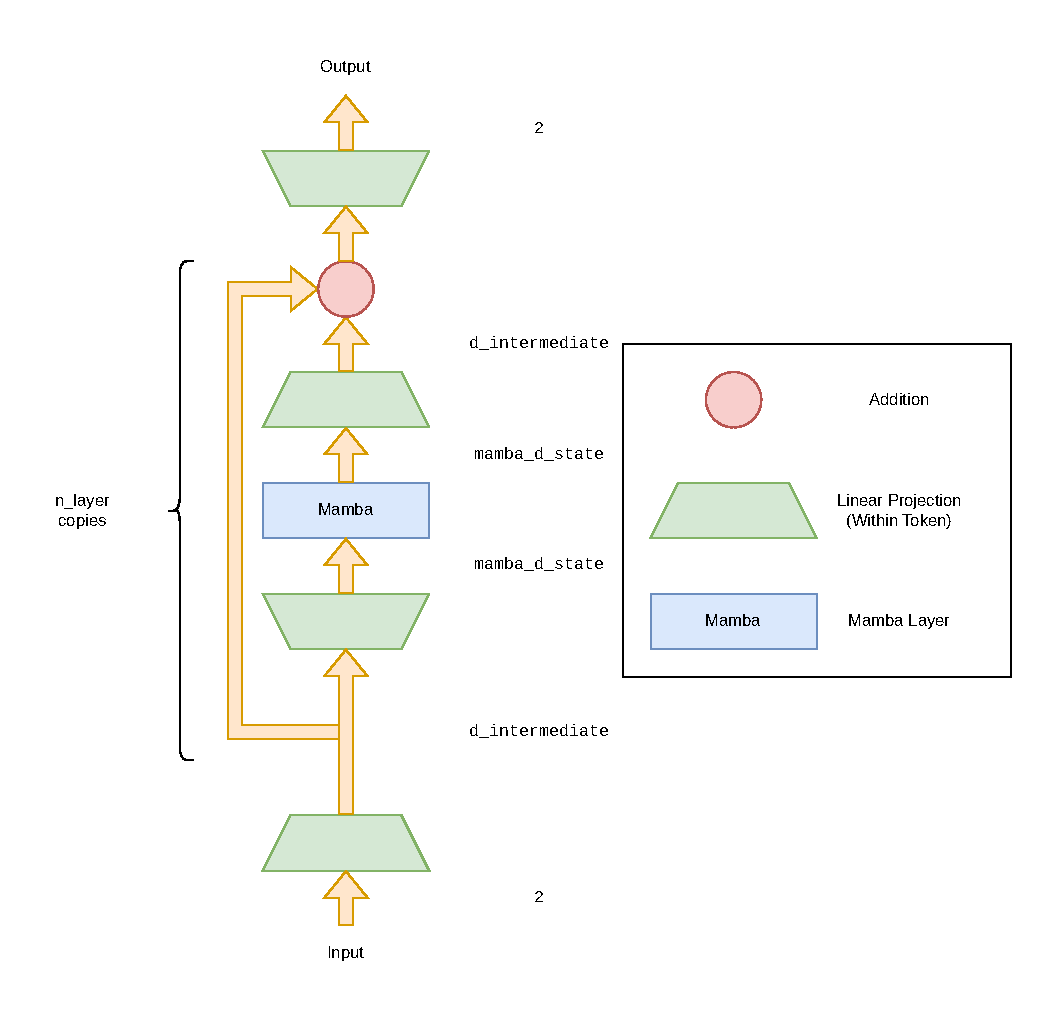
\includegraphics[width=\textwidth]{figures/sequence_stack_simple.pdf}
    \caption{Simple Mamba Stack Architecture}
    \label{simplestack}
\end{figure}

\begin{figure}
    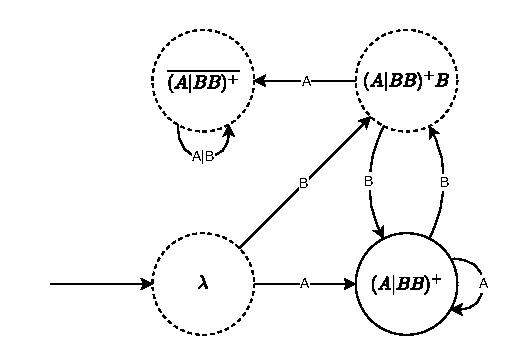
\includegraphics[width=\textwidth]{figures/a_or_bb_plus_dfa.pdf}
    \caption{DFA for \texttt{(a|bb)+}}
    \label{a_or_bb_plus_dfa}
\end{figure}


Despite their inability to perfectly predict non-star-free regular languages,
we find that Mamba is capable of recognizing certain non-star-free regular
languages with limited accuracy.

Preliminary testing on the regular language \texttt{(a|bb)+} shows a
surprisingly strong ability to recognize instances of the language, with lower
accuracy on medium-length strings.
If we construct the DFA for the language(see Figure \ref{a_or_bb_plus_dfa}), it
is clear that recognizing the language requires recognizing odd-length runs of
\verb|b|.
We hypothesize that Mamba is searching for specific odd-length runs of
\verb|b|.
If this is indeed what the model is doing, then it should achieve a nearly
perfect accuracy with member strings, since they don't contain any disqualifying
substrings, and it should struggle to get perfect accuracy with non-member
strings, since an instance might contain a disqualifying string that the model
has not learned to search for.

\textbf{Dataset} The dataset that we train Mamba to recognize is a synthetic
dataset.
The procedure for generating an instance of the dataset is as follows:
\begin{itemize}
    \item Choose a length between 1 and 64, inclusive
    \item Choose a label: either member or non-member
    \item Choose a random string that has the chosen length and label
\end{itemize}
We generate 4000 batches with 64 strings each, and train our model for 1 epoch.

\textbf{Model} The model that we train is a stack of Mamba layers with linear
projection in-between(see Figure \ref{simplestack}).
The inputs and outputs also have linear projections to make the channel numbers
match the task.
The primary hyperparameters are \verb|n_layer = 2|, \verb|mamba_d_model = 16|,
and \verb|mamba_d_state = 16|.
The rest of the hyperparameters can be found on
Github\footnote{\url{https://github.com/maxwell3025/CV-IS-Fall-2024/blob/main/mamba_formal/config/experiment_a_or_bb.yaml}}.

\textbf{Results} 
\begin{figure}
    \begin{subfigure}{0.5\textwidth}
        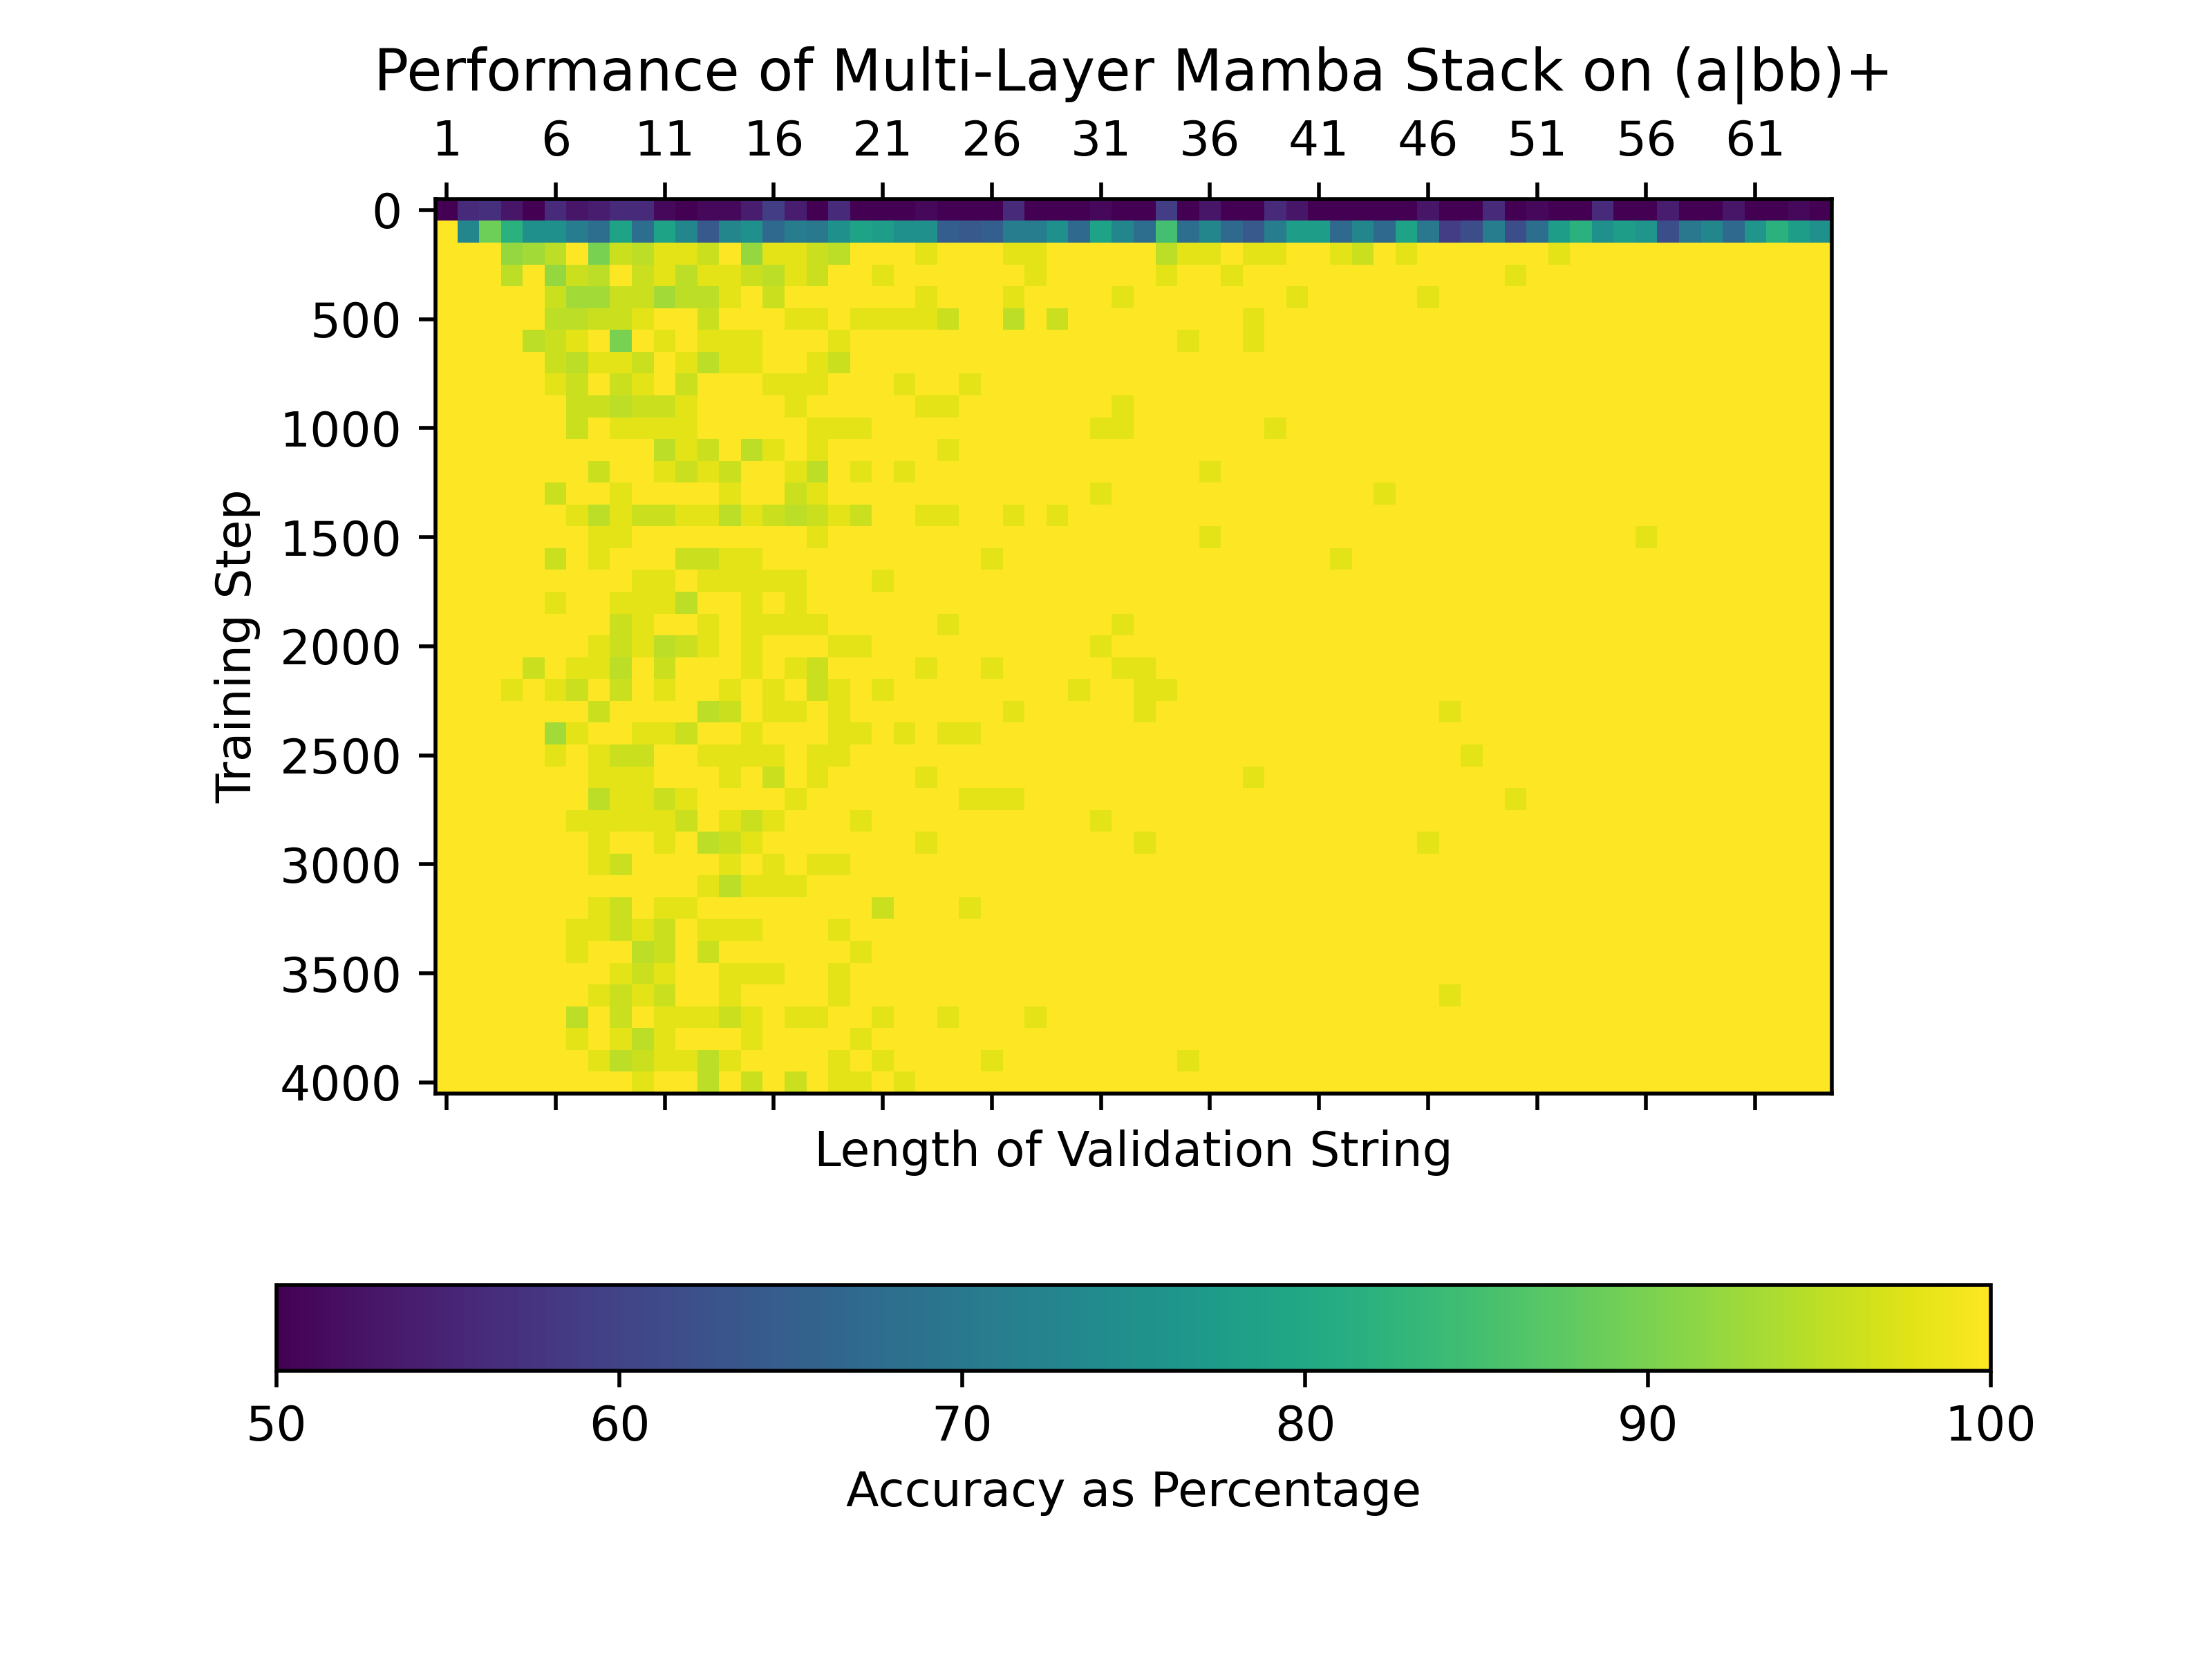
\includegraphics[width=\textwidth]{figures/a_or_bb_plus_mixed.png}
        \caption{}
    \end{subfigure}
    \begin{subfigure}{0.5\textwidth}
        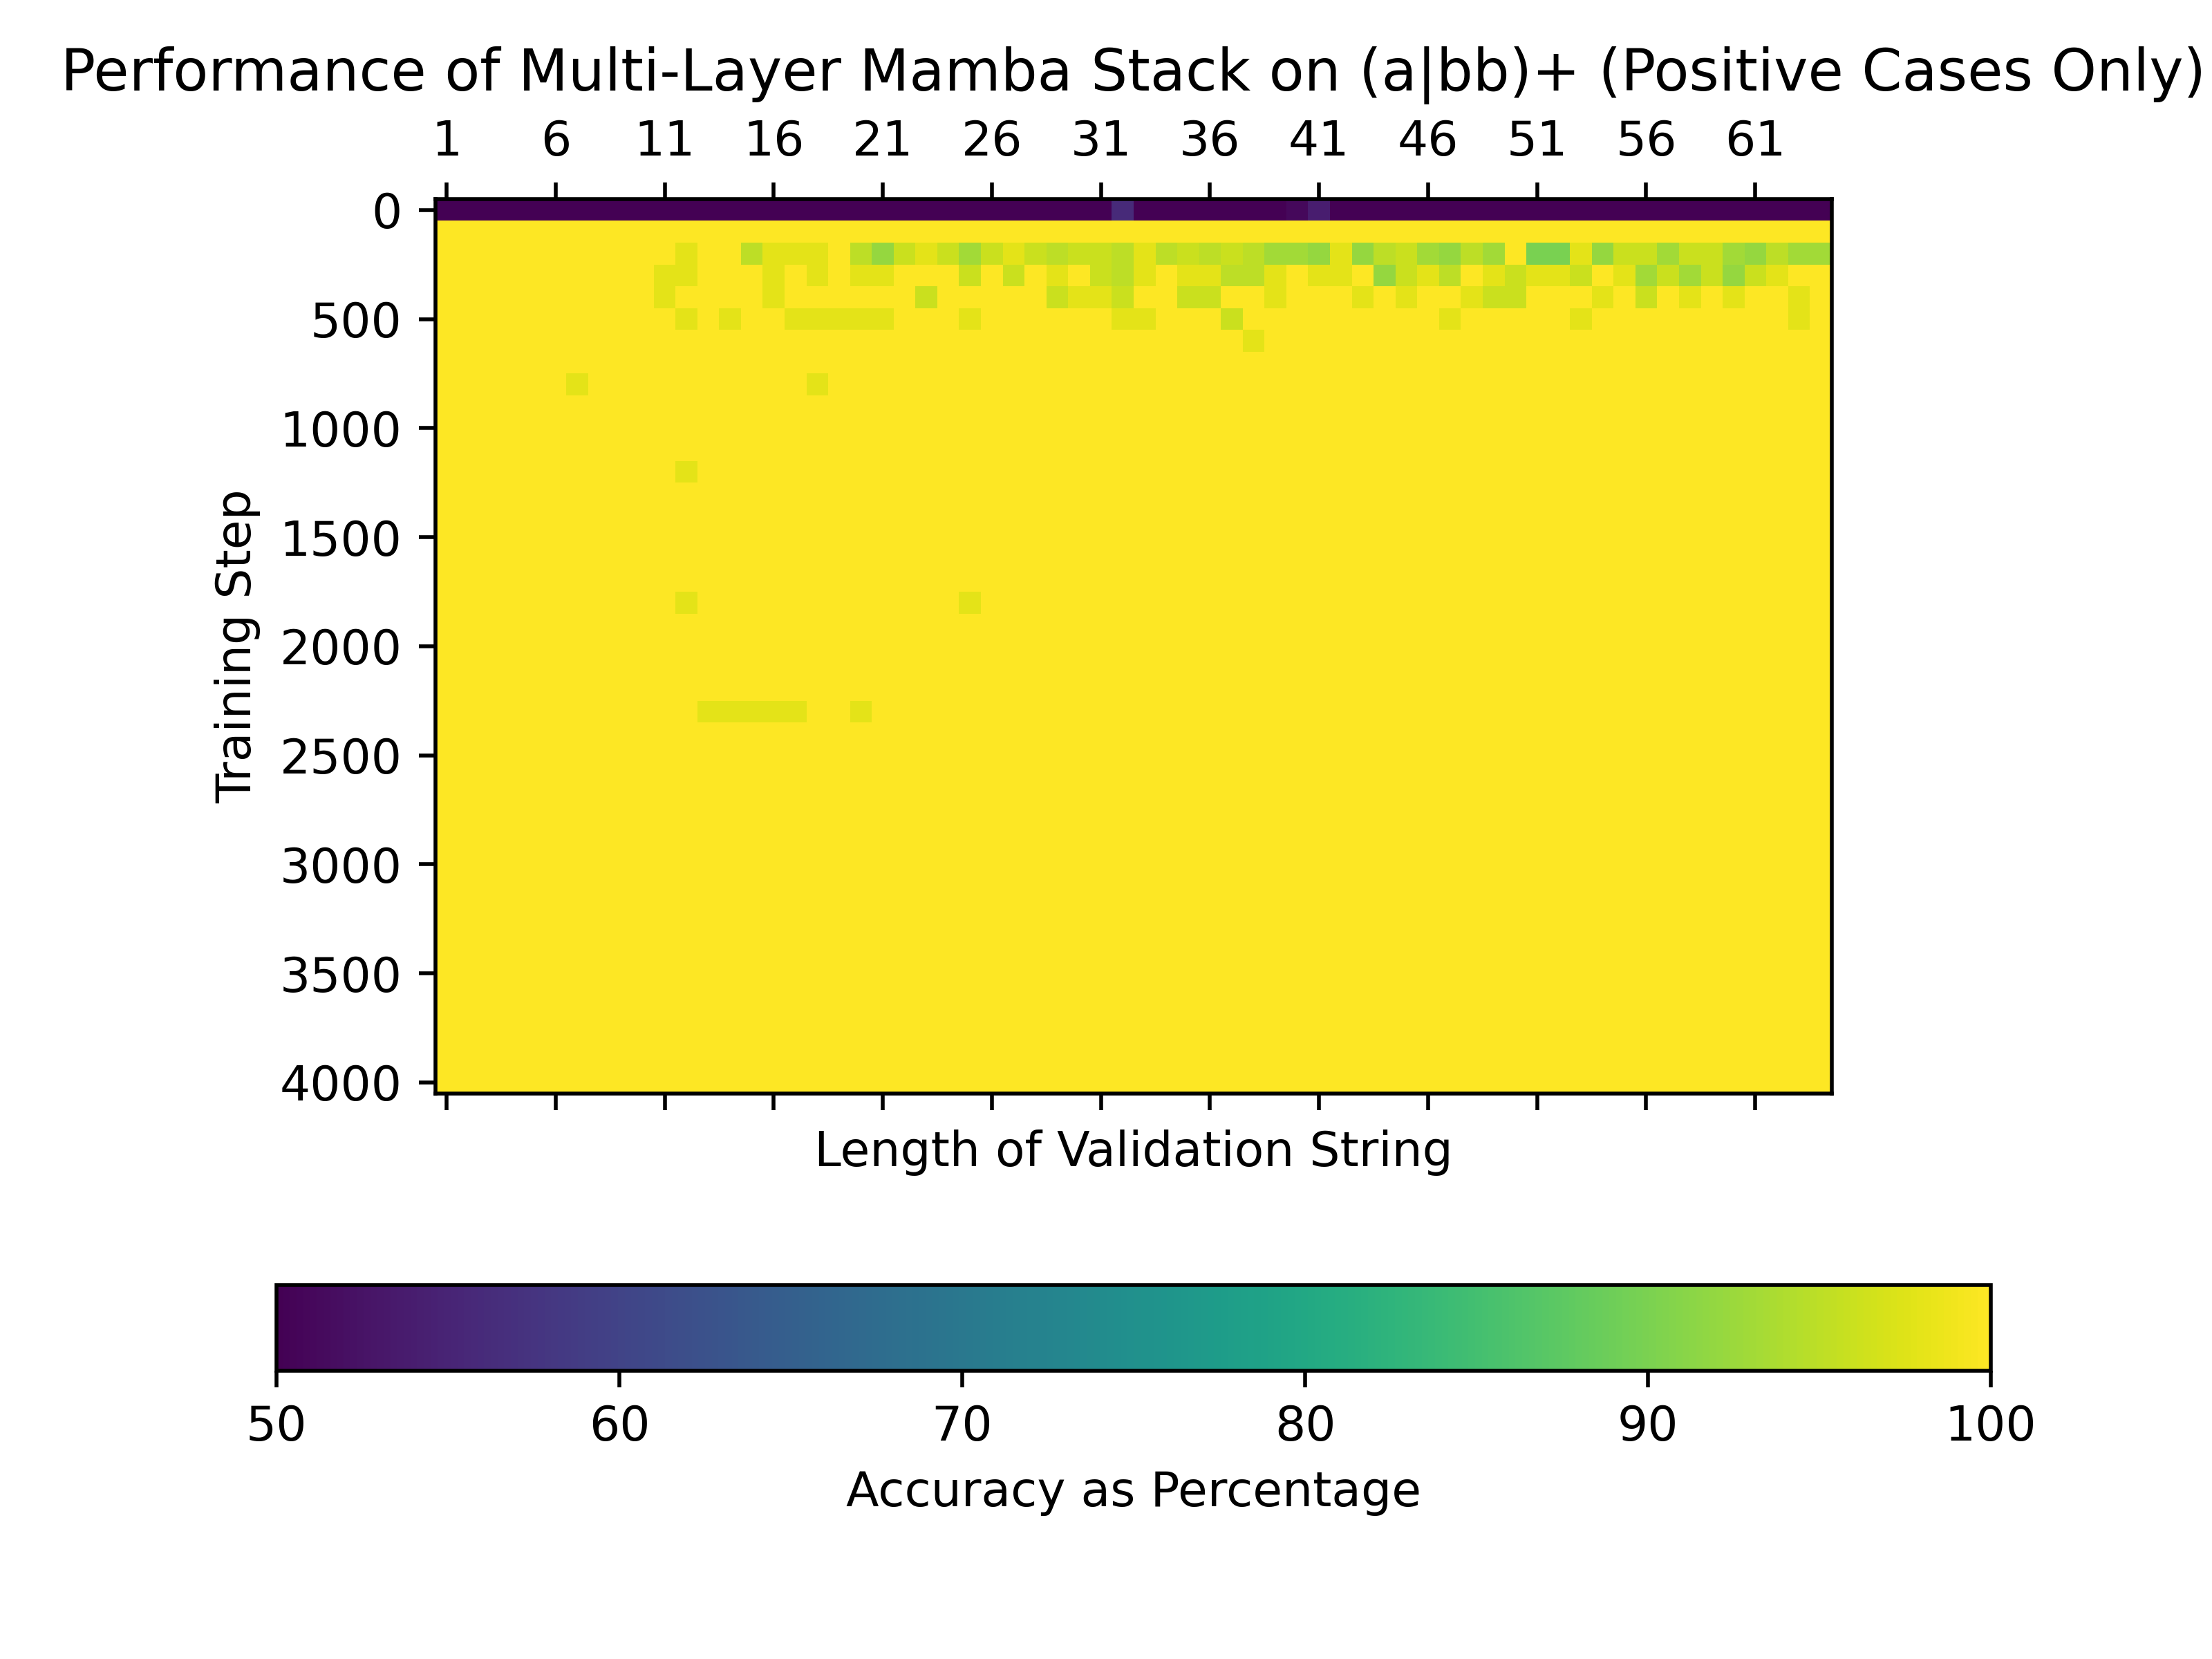
\includegraphics[width=\textwidth]{figures/a_or_bb_plus_positive_only.png}
        \caption{}
    \end{subfigure}
    \caption{Results for \texttt{a|bb+}}
\end{figure}
We find that the model quickly attains nearly perfect performance on positive
cases, with the trained model only making errors with negative cases.
This strongly suggests that our hypothesis is true.
The model is correctly identifying that positive cases lack the forbidden
strings that the model memorized, and the model is failing to recognize some
negative cases, since they contain odd-length forbidden strings that were not
memorized.

\subsection{Formation of "Bad Habits" with Mamba}
Given Mamba's limited ability to recognize regular languages, it would be useful
to place it alongside more formally powerful models such as LSTMs, which can
trivially model general regular languages given large enough
parameters\cite{lstmformal}. Unfortunately, preliminary testing found that the
inclusion of Mamba in series with LSTMs leads to a degradation of generalization
ability.

We suspect that this explains the inclusion of drop-path in many Mamba-based
architectures.
Drop-path is a normalization layer introduced by FractalNet\cite{fractalnet} in
which the outputs of entire layers in an architecture are set to zero.
As stated by the authors, this trains the model to do the task without certain
components.
In the literature, we find that machine learning architectures like
MedMamba\cite{medmamba}, VMamba\cite{vmamba}, and MambaND\cite{mamband} apply
drop-path to the output of Mamba layers.
We suspect this is done since Mamba learns certain tasks very quickly, leading to
the derivatives produced by Mamba to "drown out" the derivatives coming from the
other layers.
Drop-path would then allow the other layers to learn to solve the tasks without
being influenced by the Mamba layer.

In order to confirm these findings, we test a mixed Mamba model to solve a task
that Mamba alone cannot solve.

It has been shown that Mamba cannot recognize even bitstrings\cite{ssmformal},
a finding we confirm in our own preliminary testing, while parity has been shown
to be a trivial task for LSTM architectures, a finding that we again reproduce
in our own testing.

\textbf{Model} Our model in this test is identical to the model shown in
Figure \ref{simplestack}, except that 2 input layers are replaced with LSTM
layers.
In addition, drop path layers are placed after each Mamba layer.

\textbf{Dataset}
The dataset that we use is exactly the same as the one used in the previous
experiment, except that instead of sampling the language \texttt{a|bb+},
we sample the language \texttt{(0*10*10*)*}, or the language of even bitstrings.

\textbf{Results}
\begin{figure}
    \begin{subfigure}{0.5\textwidth}
        \begin{center}
        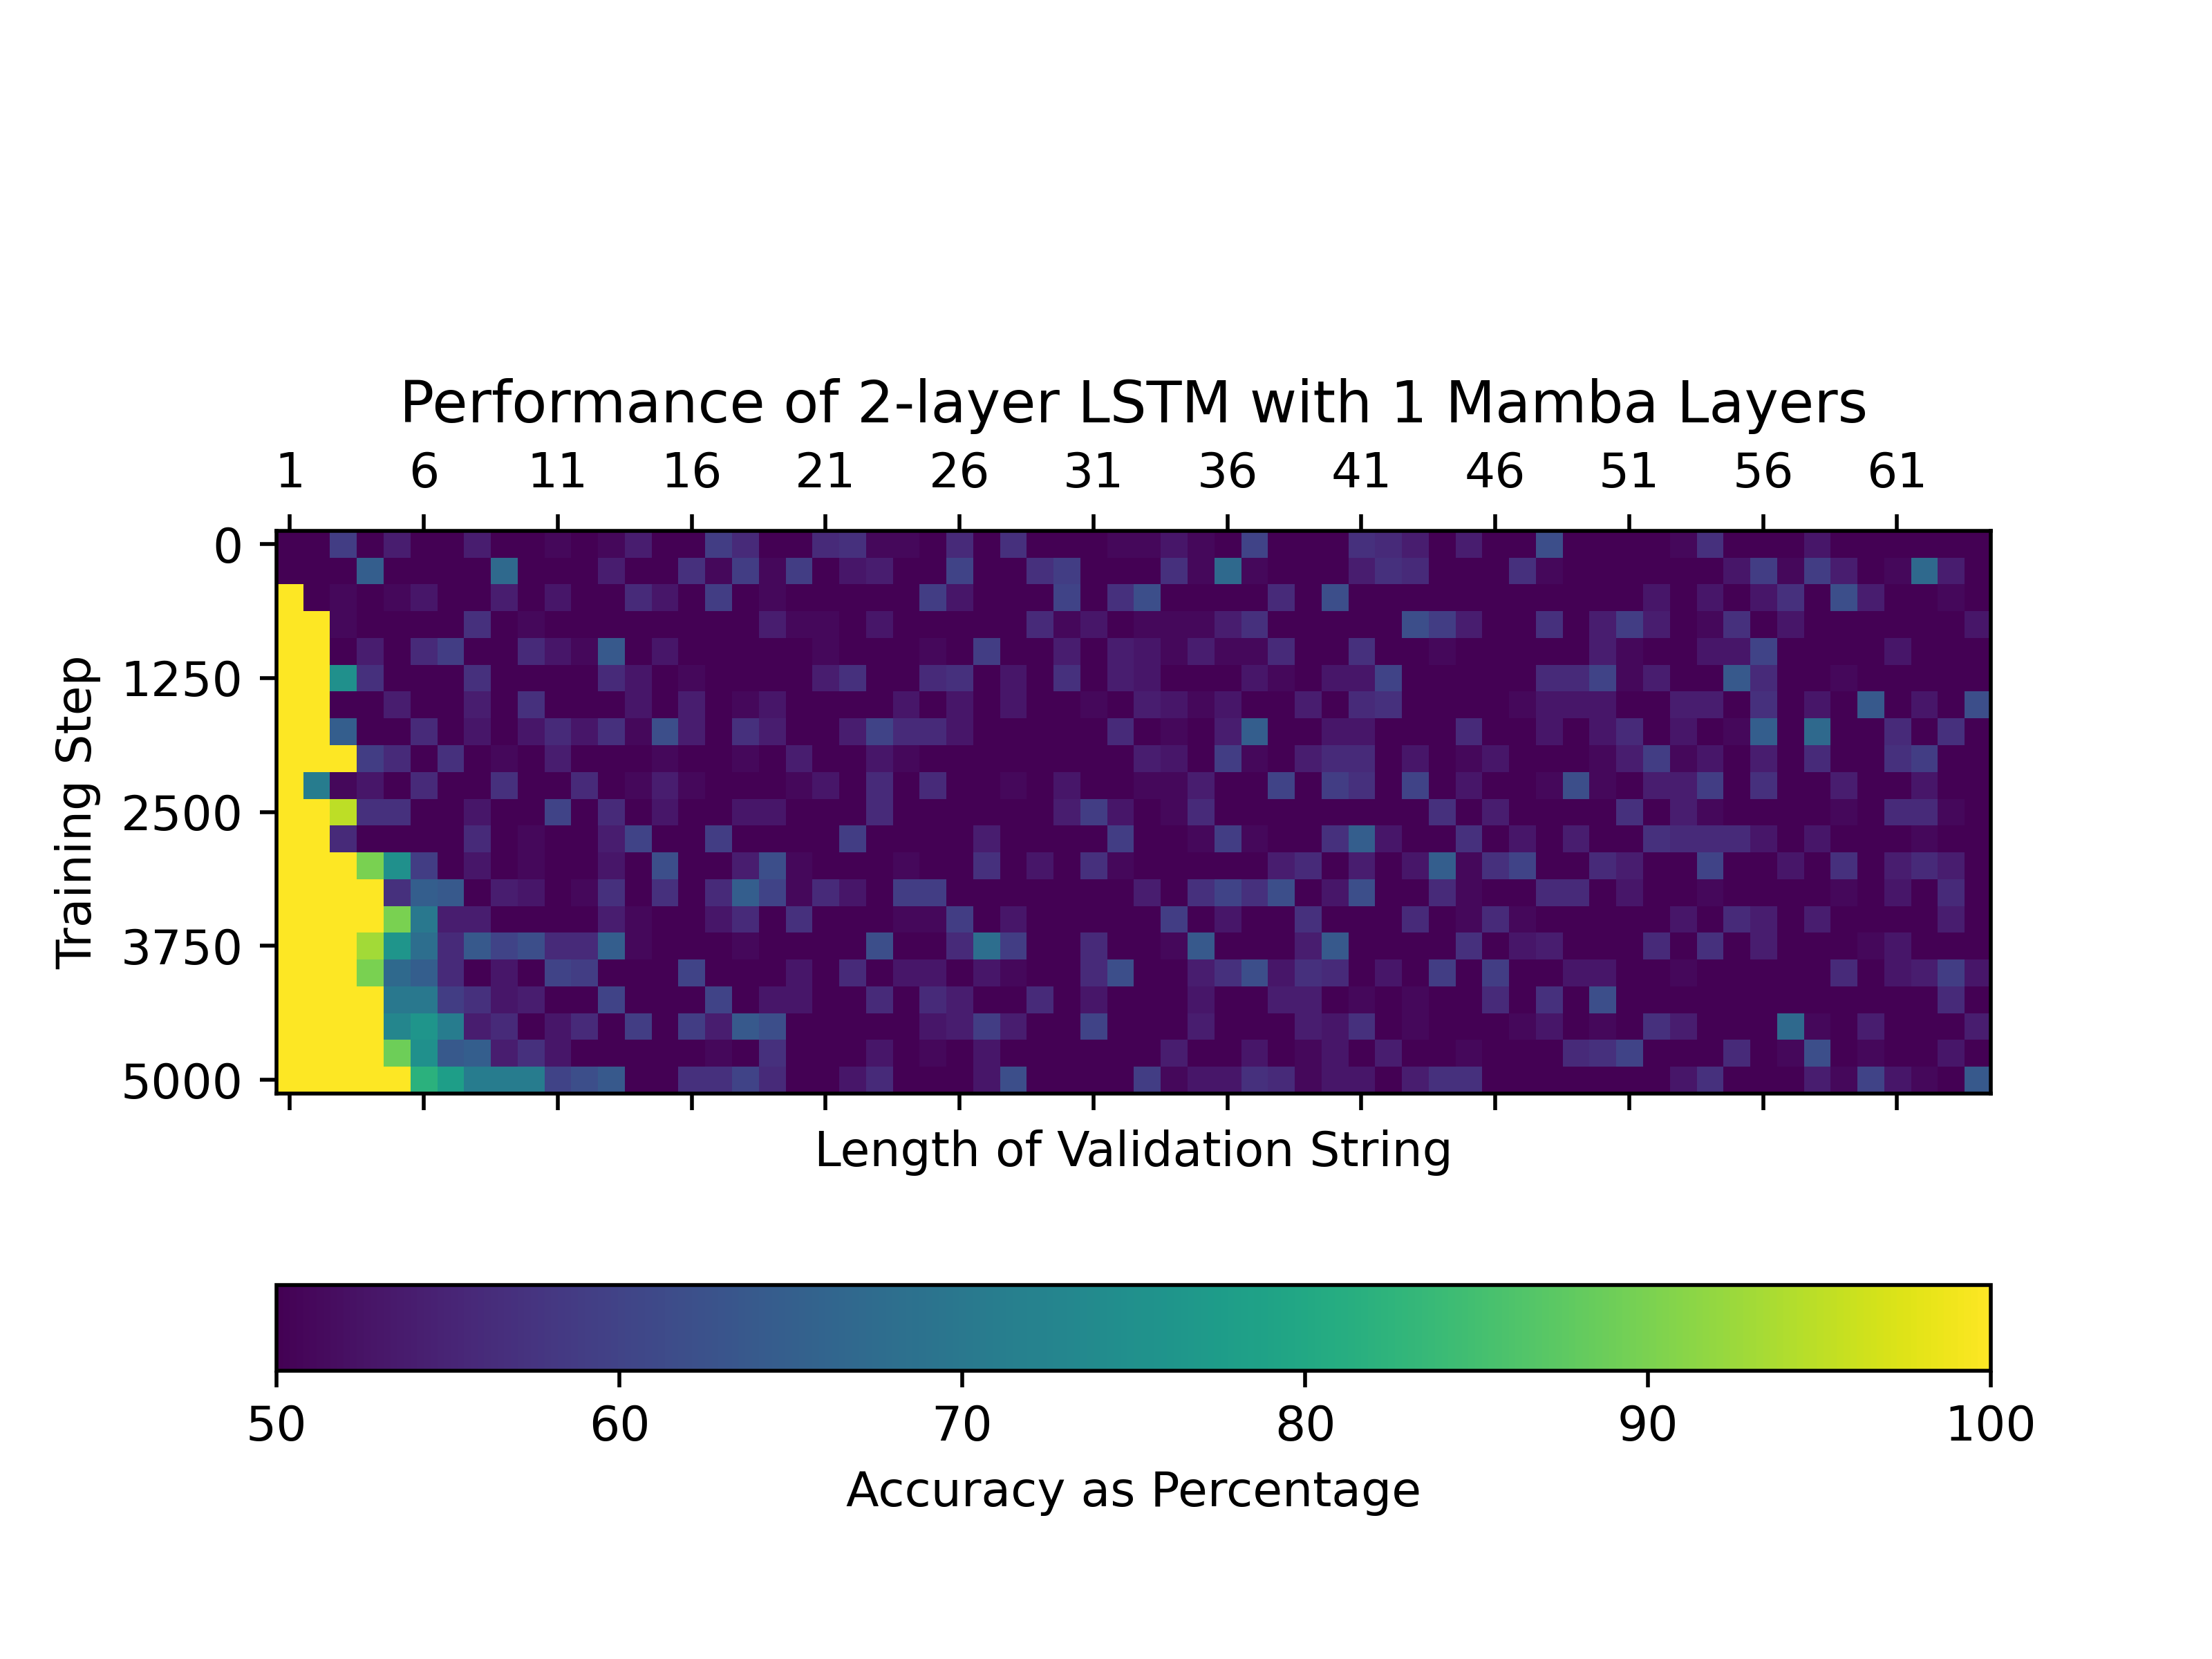
\includegraphics[width=0.8\textwidth]{figures/parity_lstm_False_3_1.png.png}
        \end{center}
    \end{subfigure}\begin{subfigure}{0.5\textwidth}
        \begin{center}
        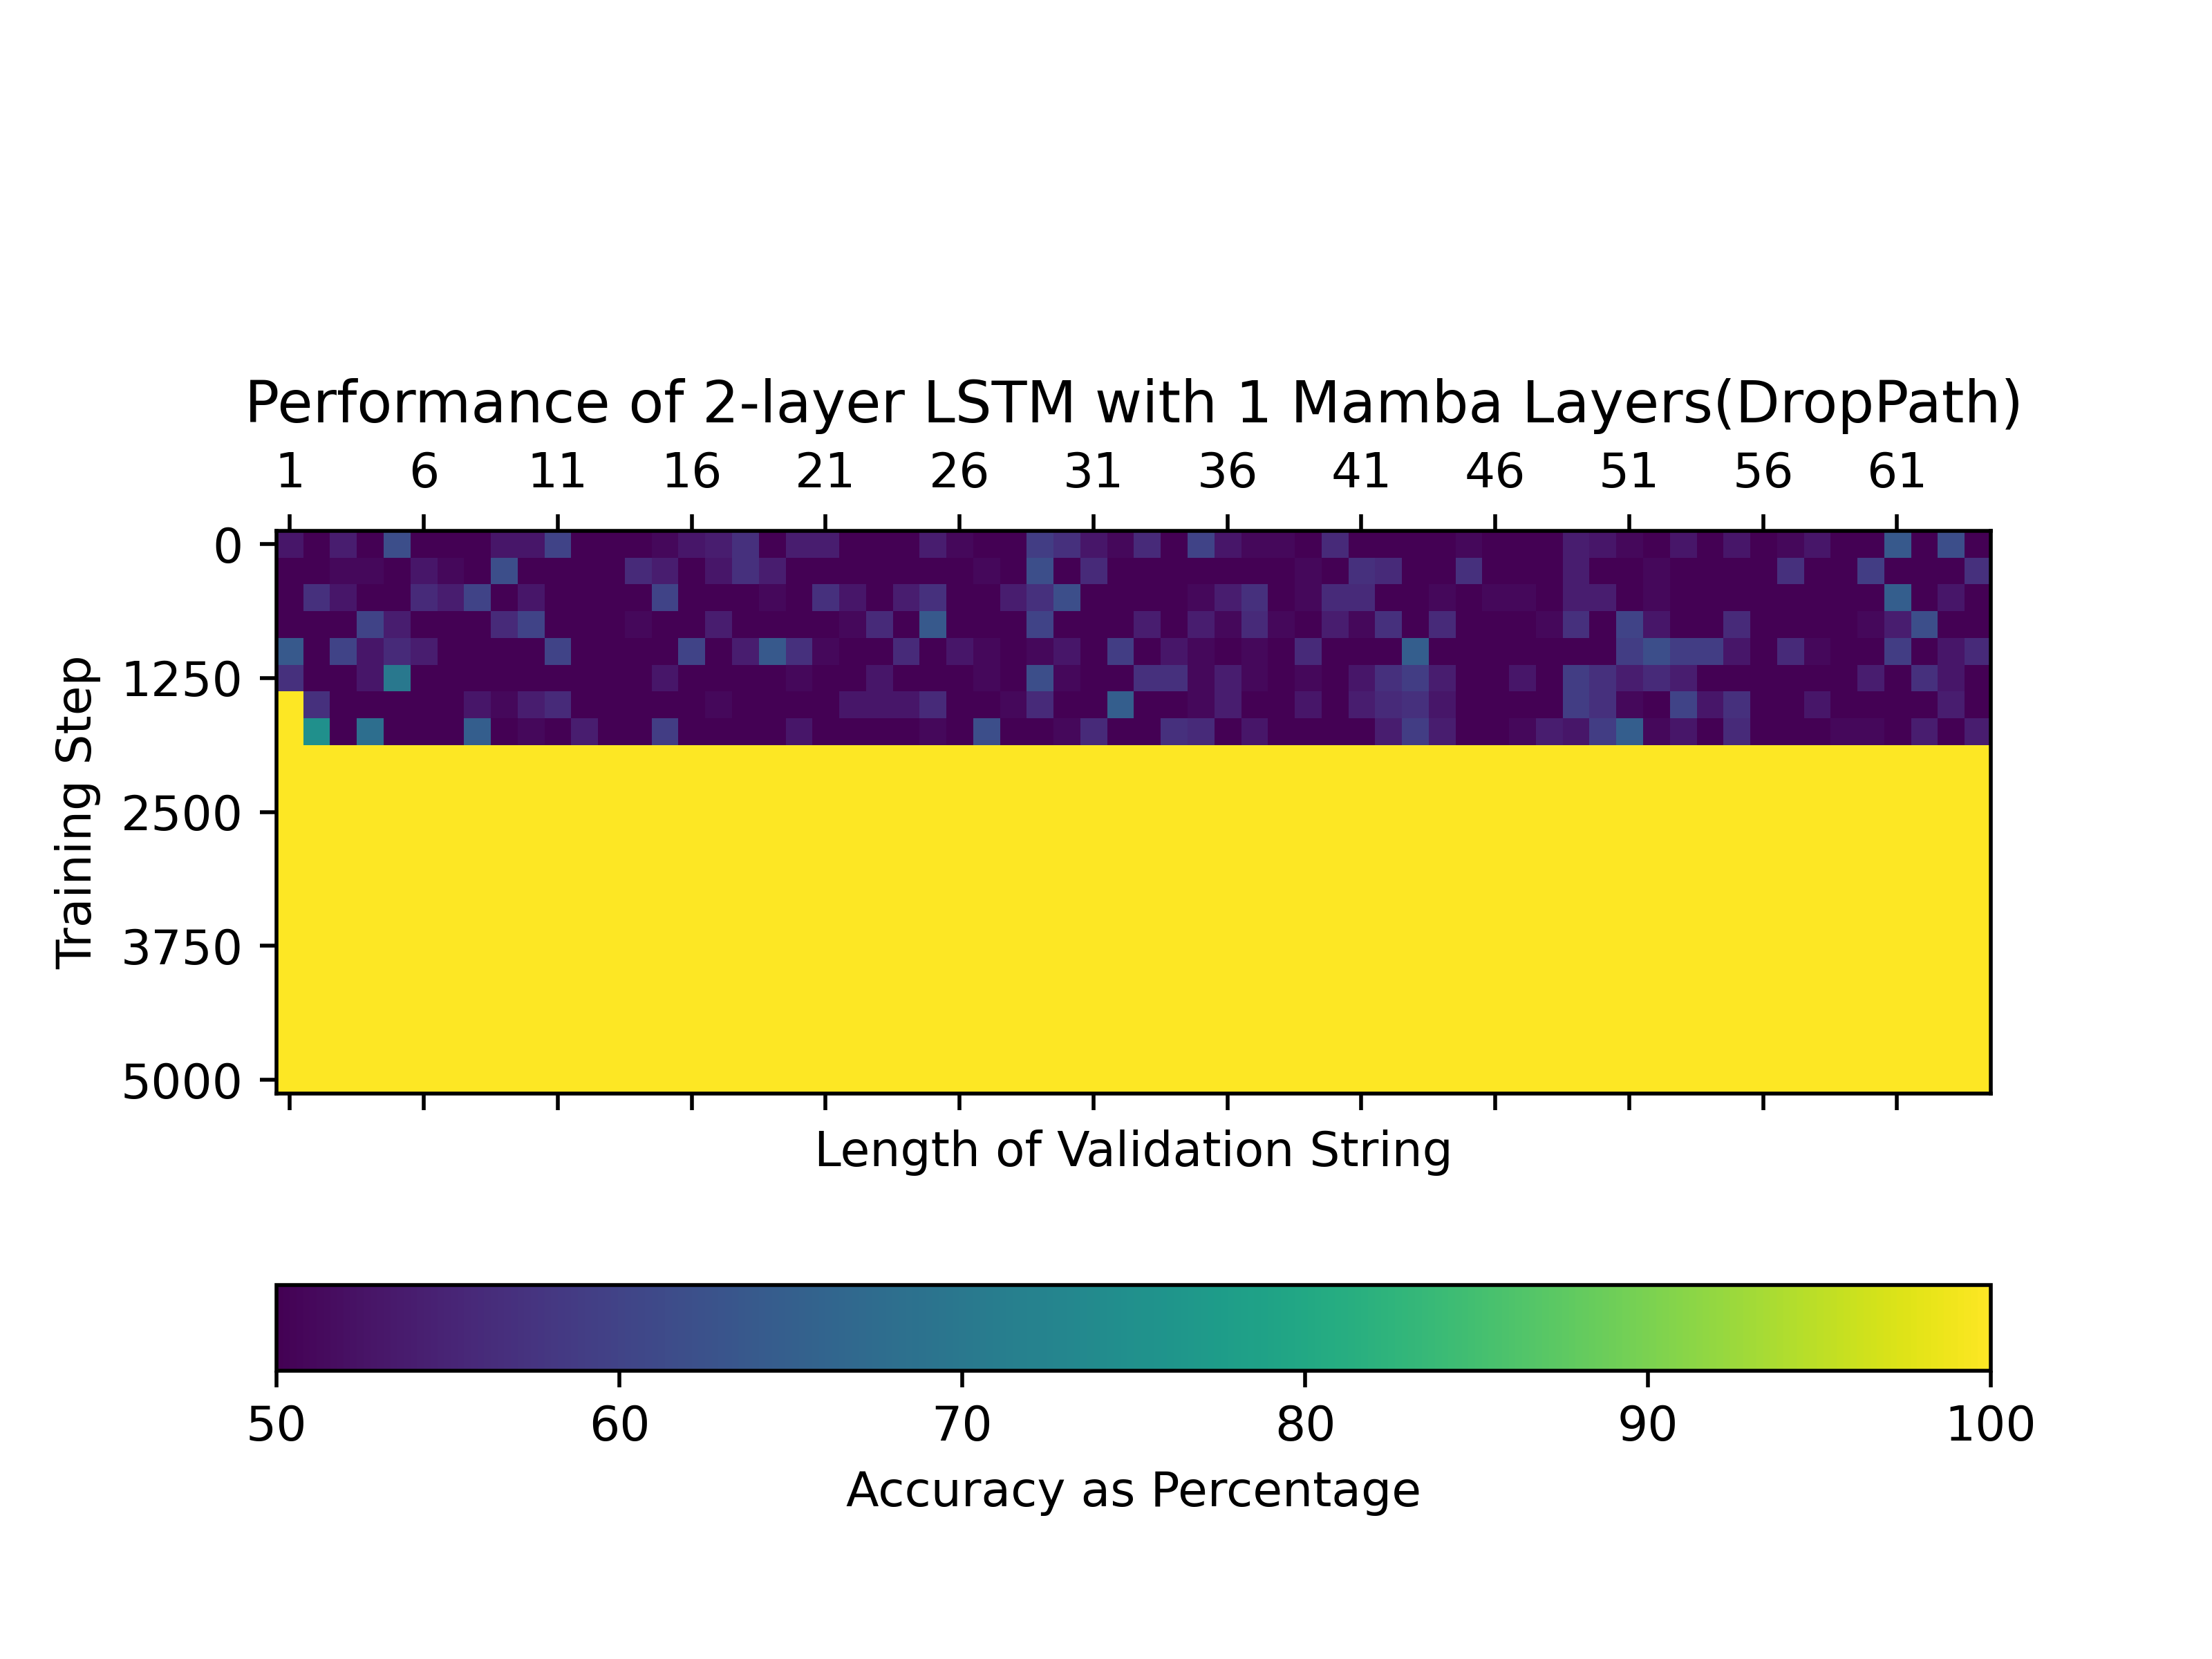
\includegraphics[width=0.8\textwidth]{figures/parity_lstm_True_3_1.png.png}
        \end{center}
    \end{subfigure}
    \begin{subfigure}{0.5\textwidth}
        \begin{center}
        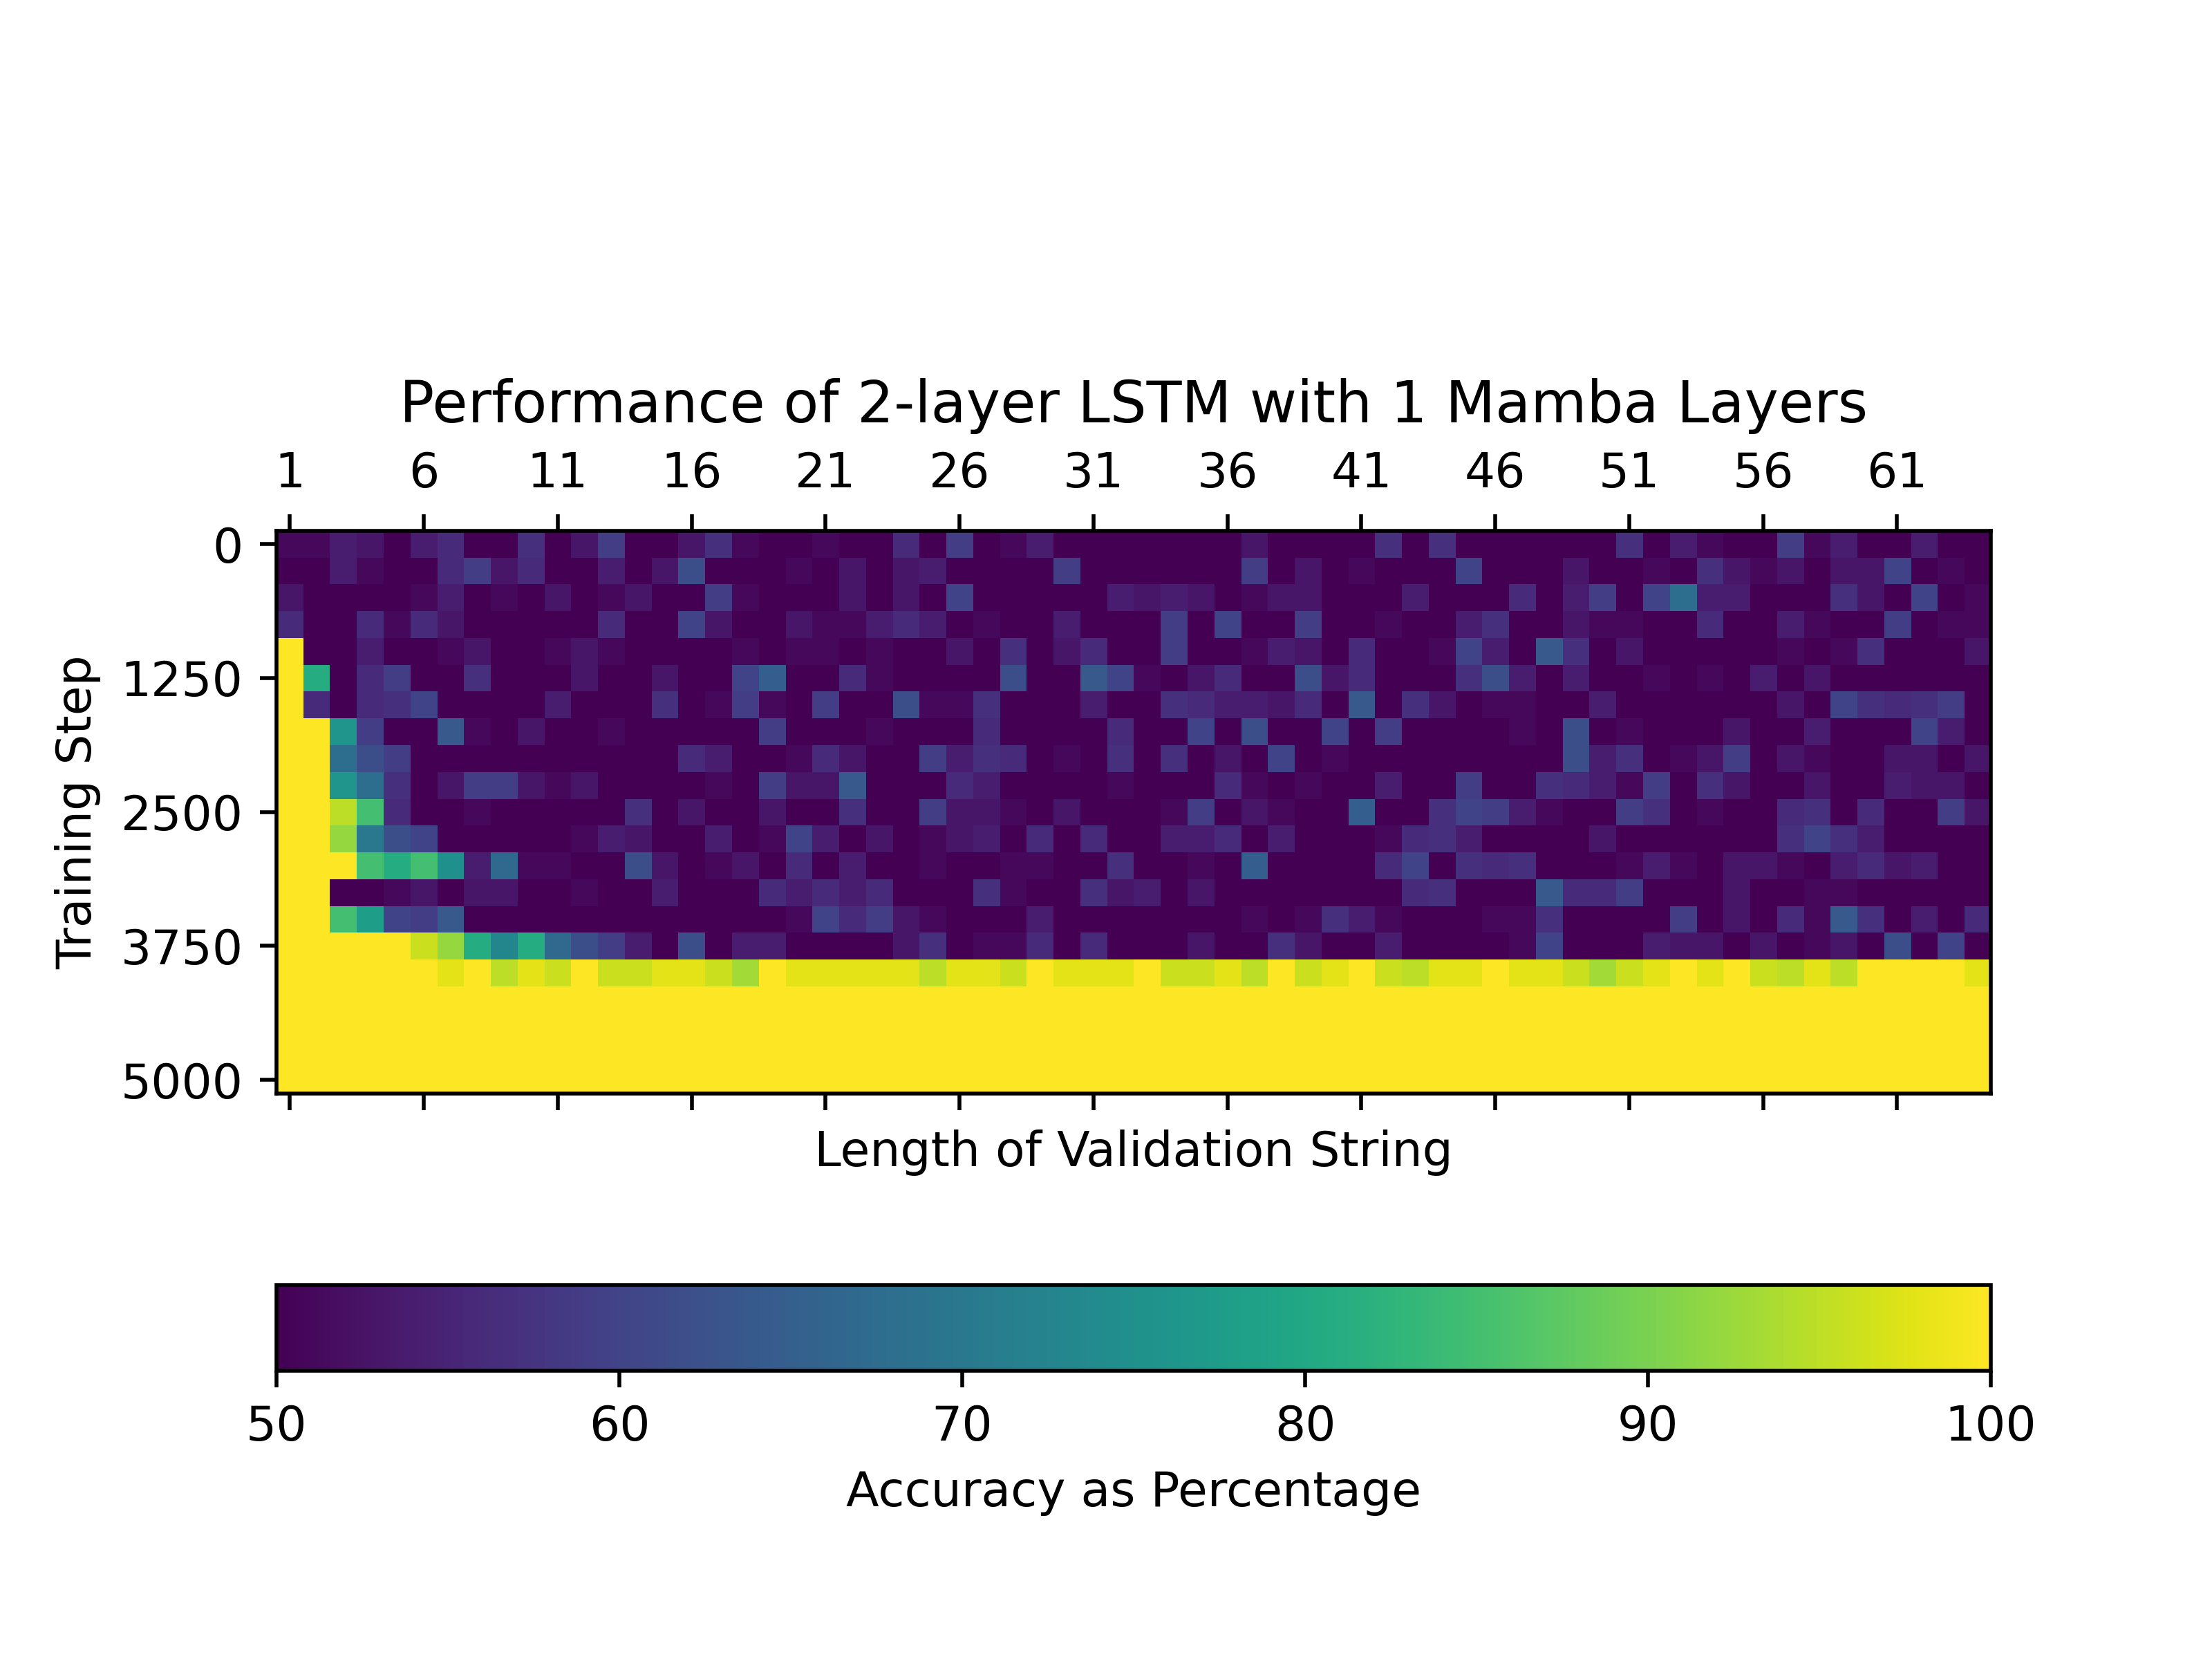
\includegraphics[width=0.8\textwidth]{figures/parity_lstm_False_3_2.png.png}
        \end{center}
    \end{subfigure}\begin{subfigure}{0.5\textwidth}
        \begin{center}
        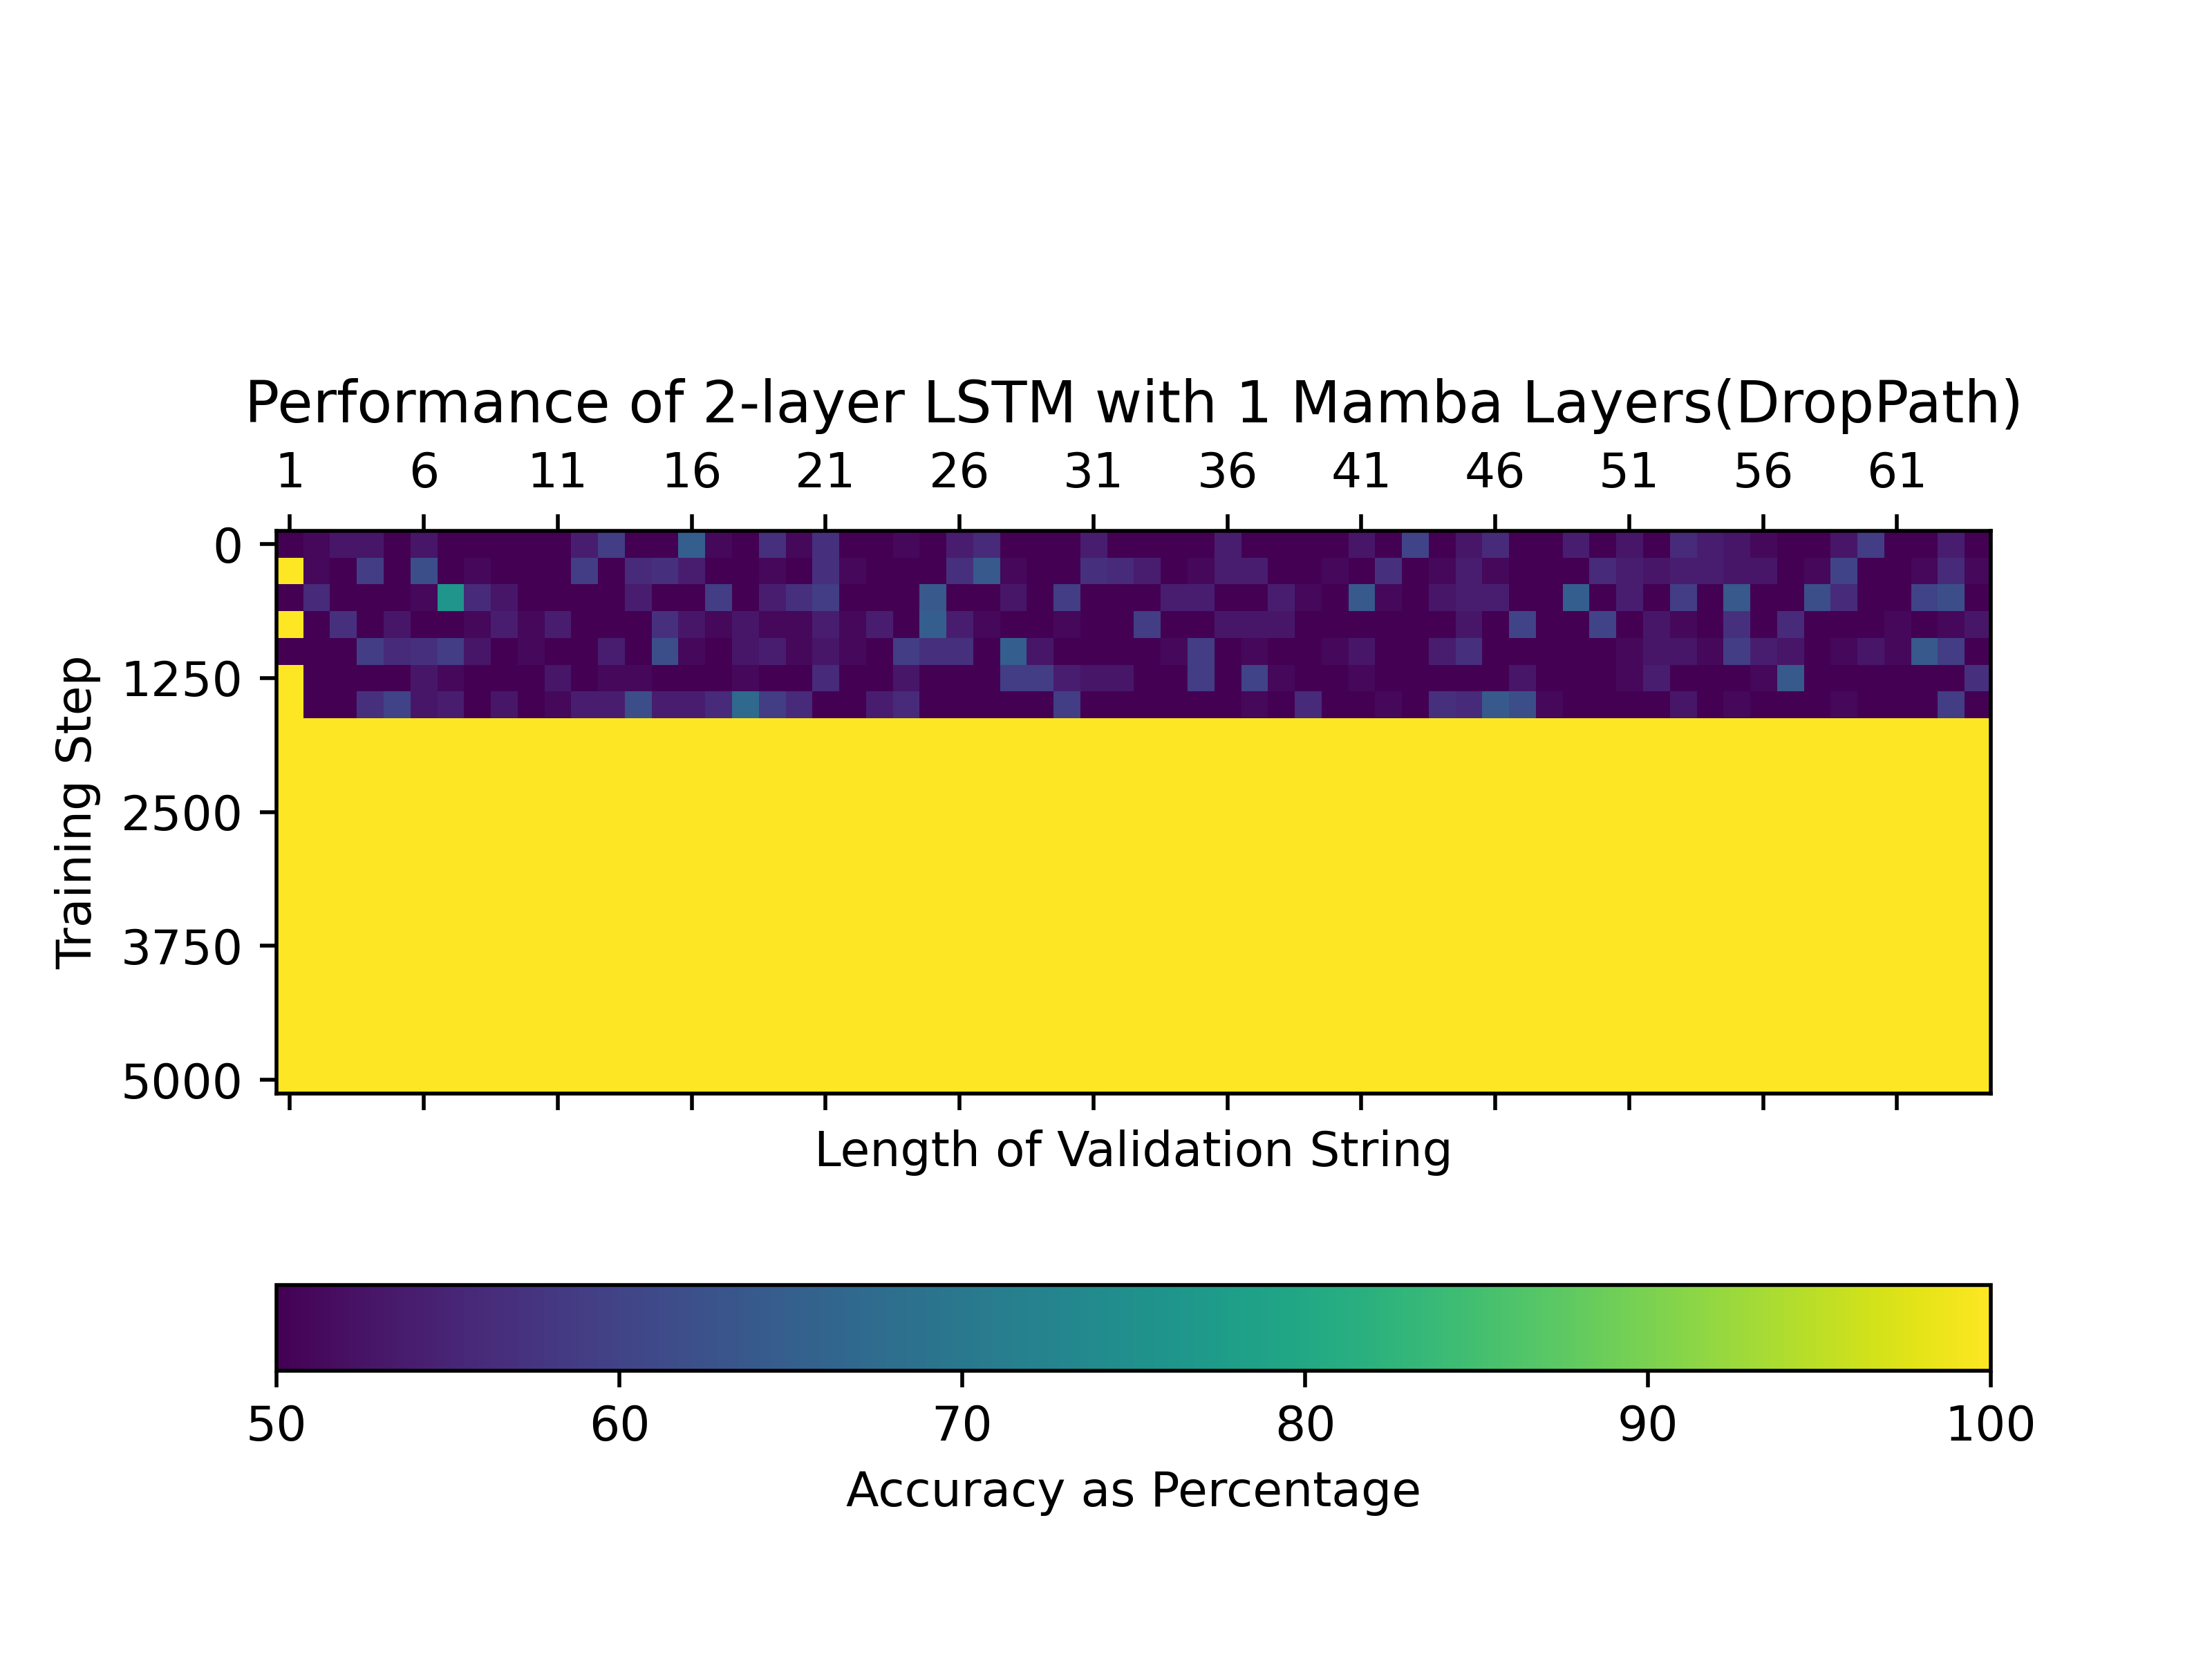
\includegraphics[width=0.8\textwidth]{figures/parity_lstm_True_3_2.png.png}
        \end{center}
    \end{subfigure}
    \begin{subfigure}{0.5\textwidth}
        \begin{center}
        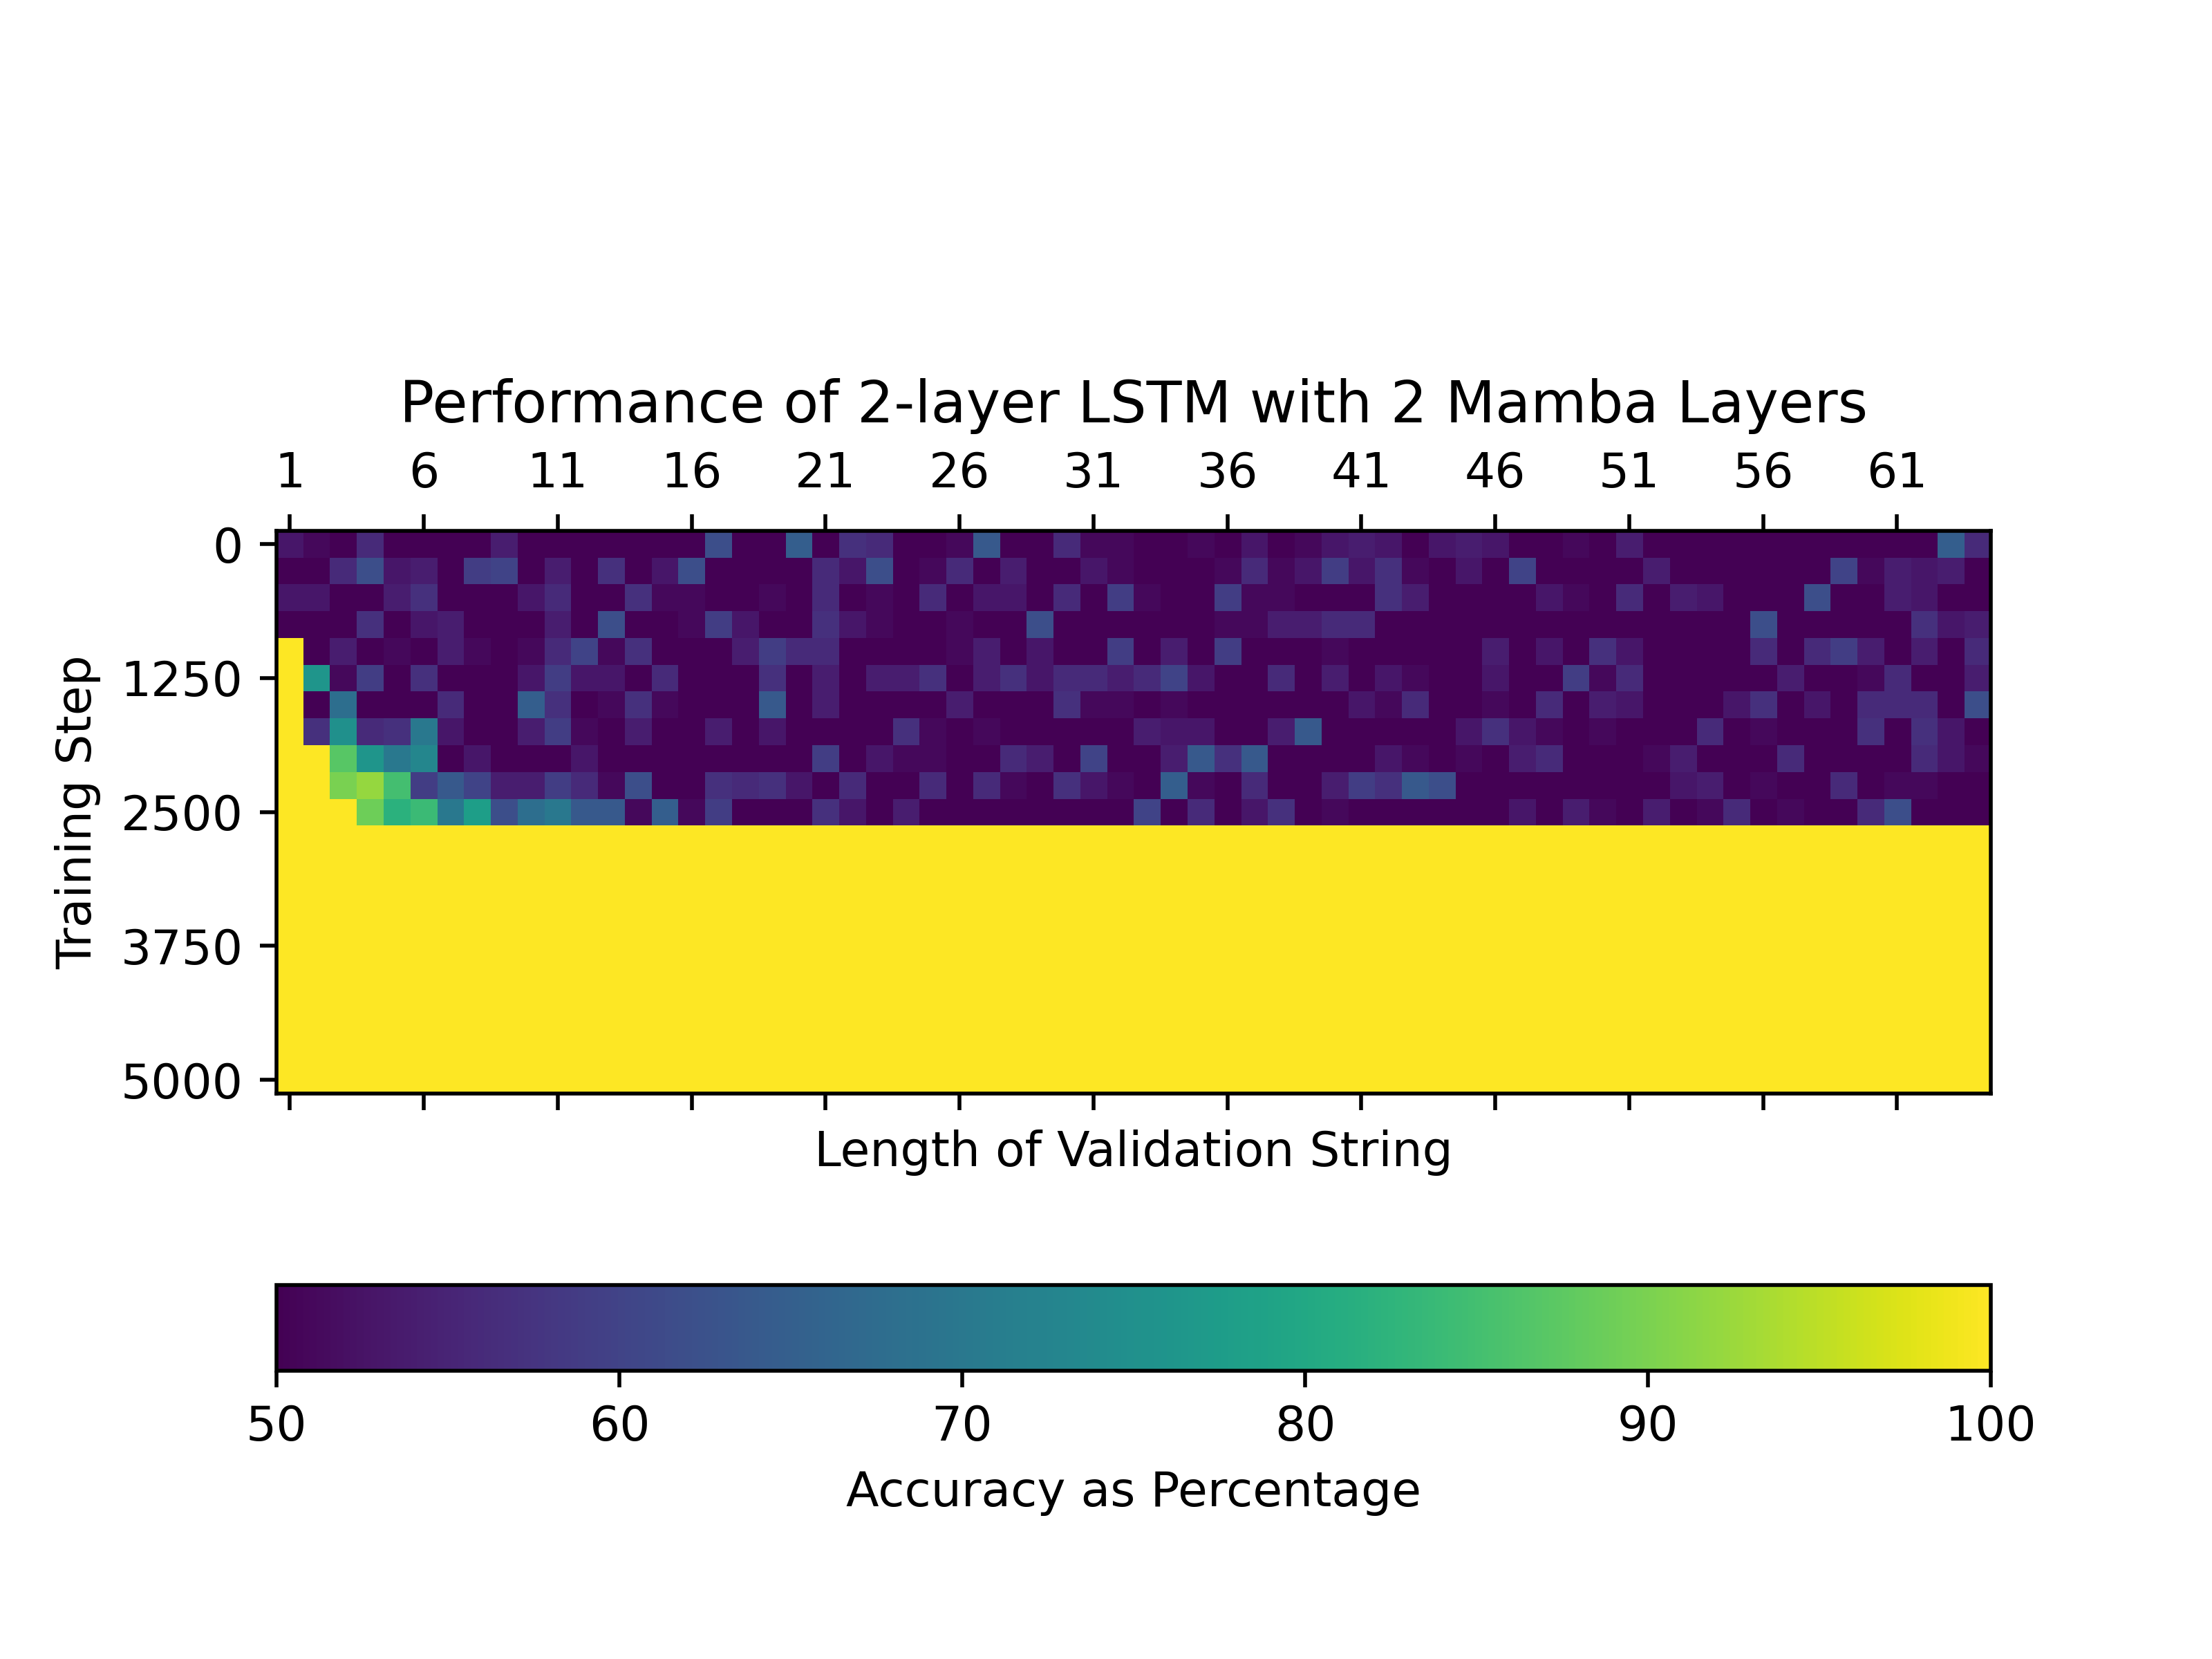
\includegraphics[width=0.8\textwidth]{figures/parity_lstm_False_4_1.png.png}
        \end{center}
    \end{subfigure}\begin{subfigure}{0.5\textwidth}
        \begin{center}
        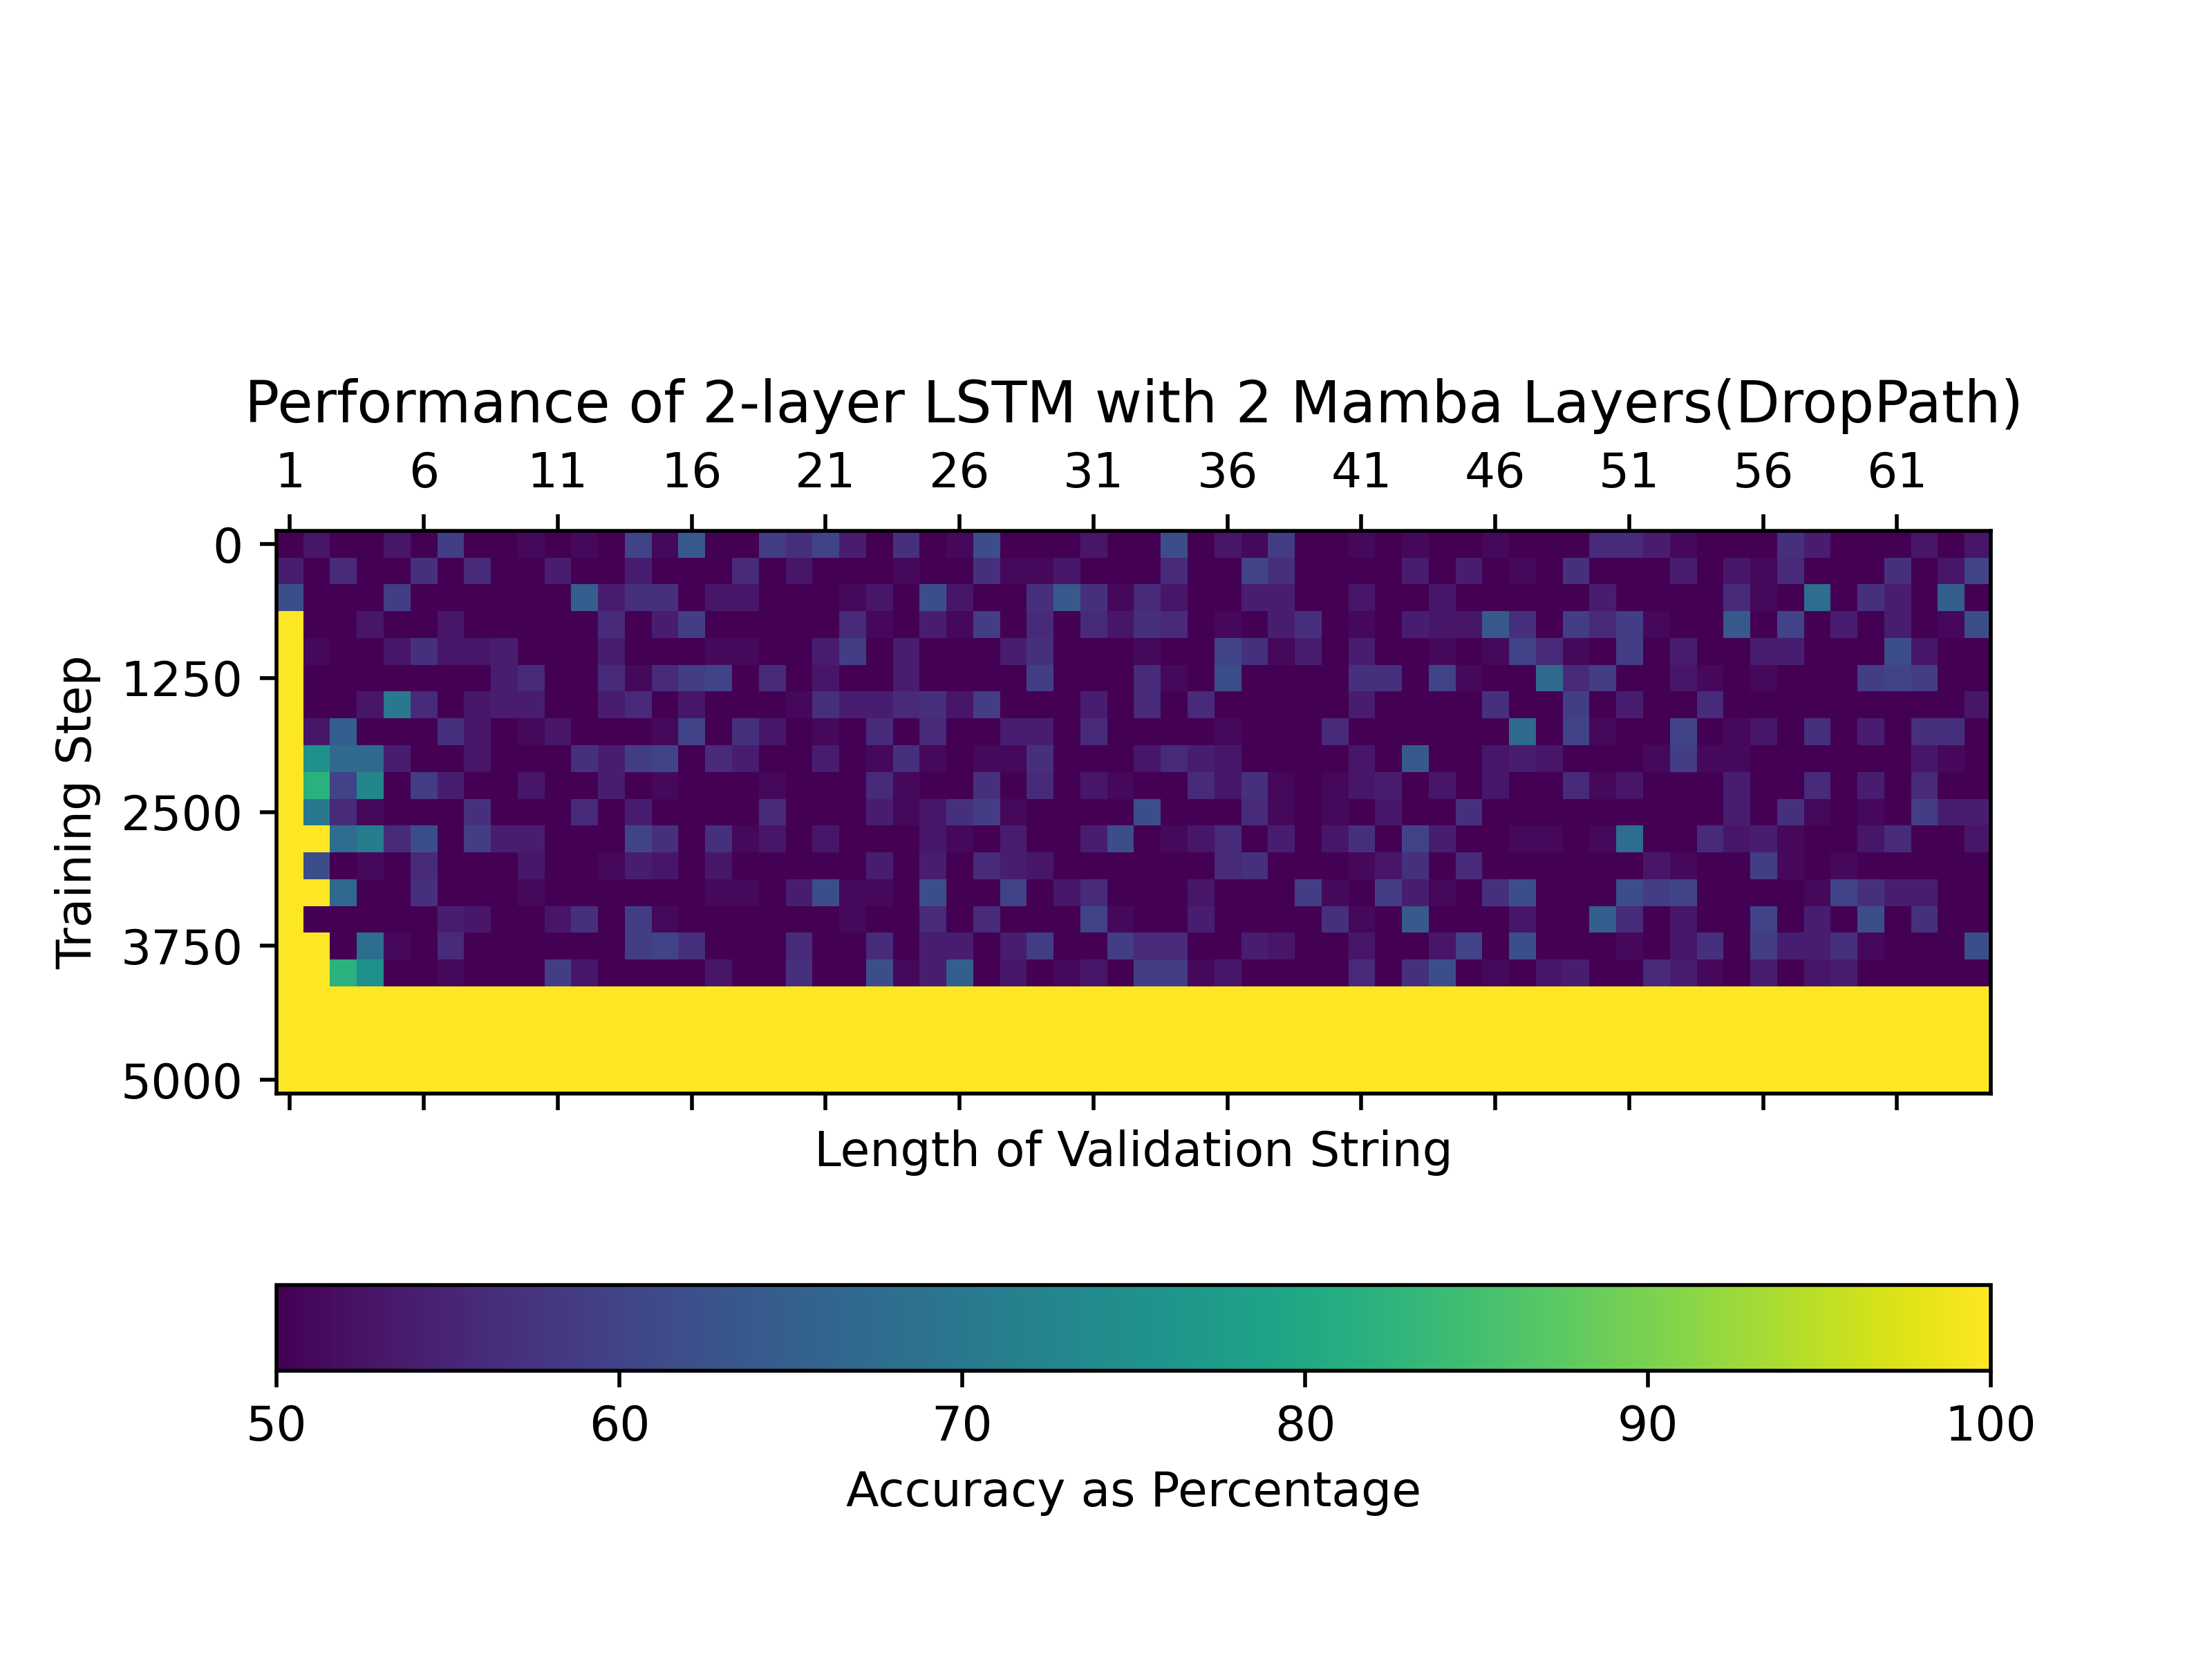
\includegraphics[width=0.8\textwidth]{figures/parity_lstm_True_4_1.png.png}
        \end{center}
    \end{subfigure}
    \begin{subfigure}{0.5\textwidth}
        \begin{center}
        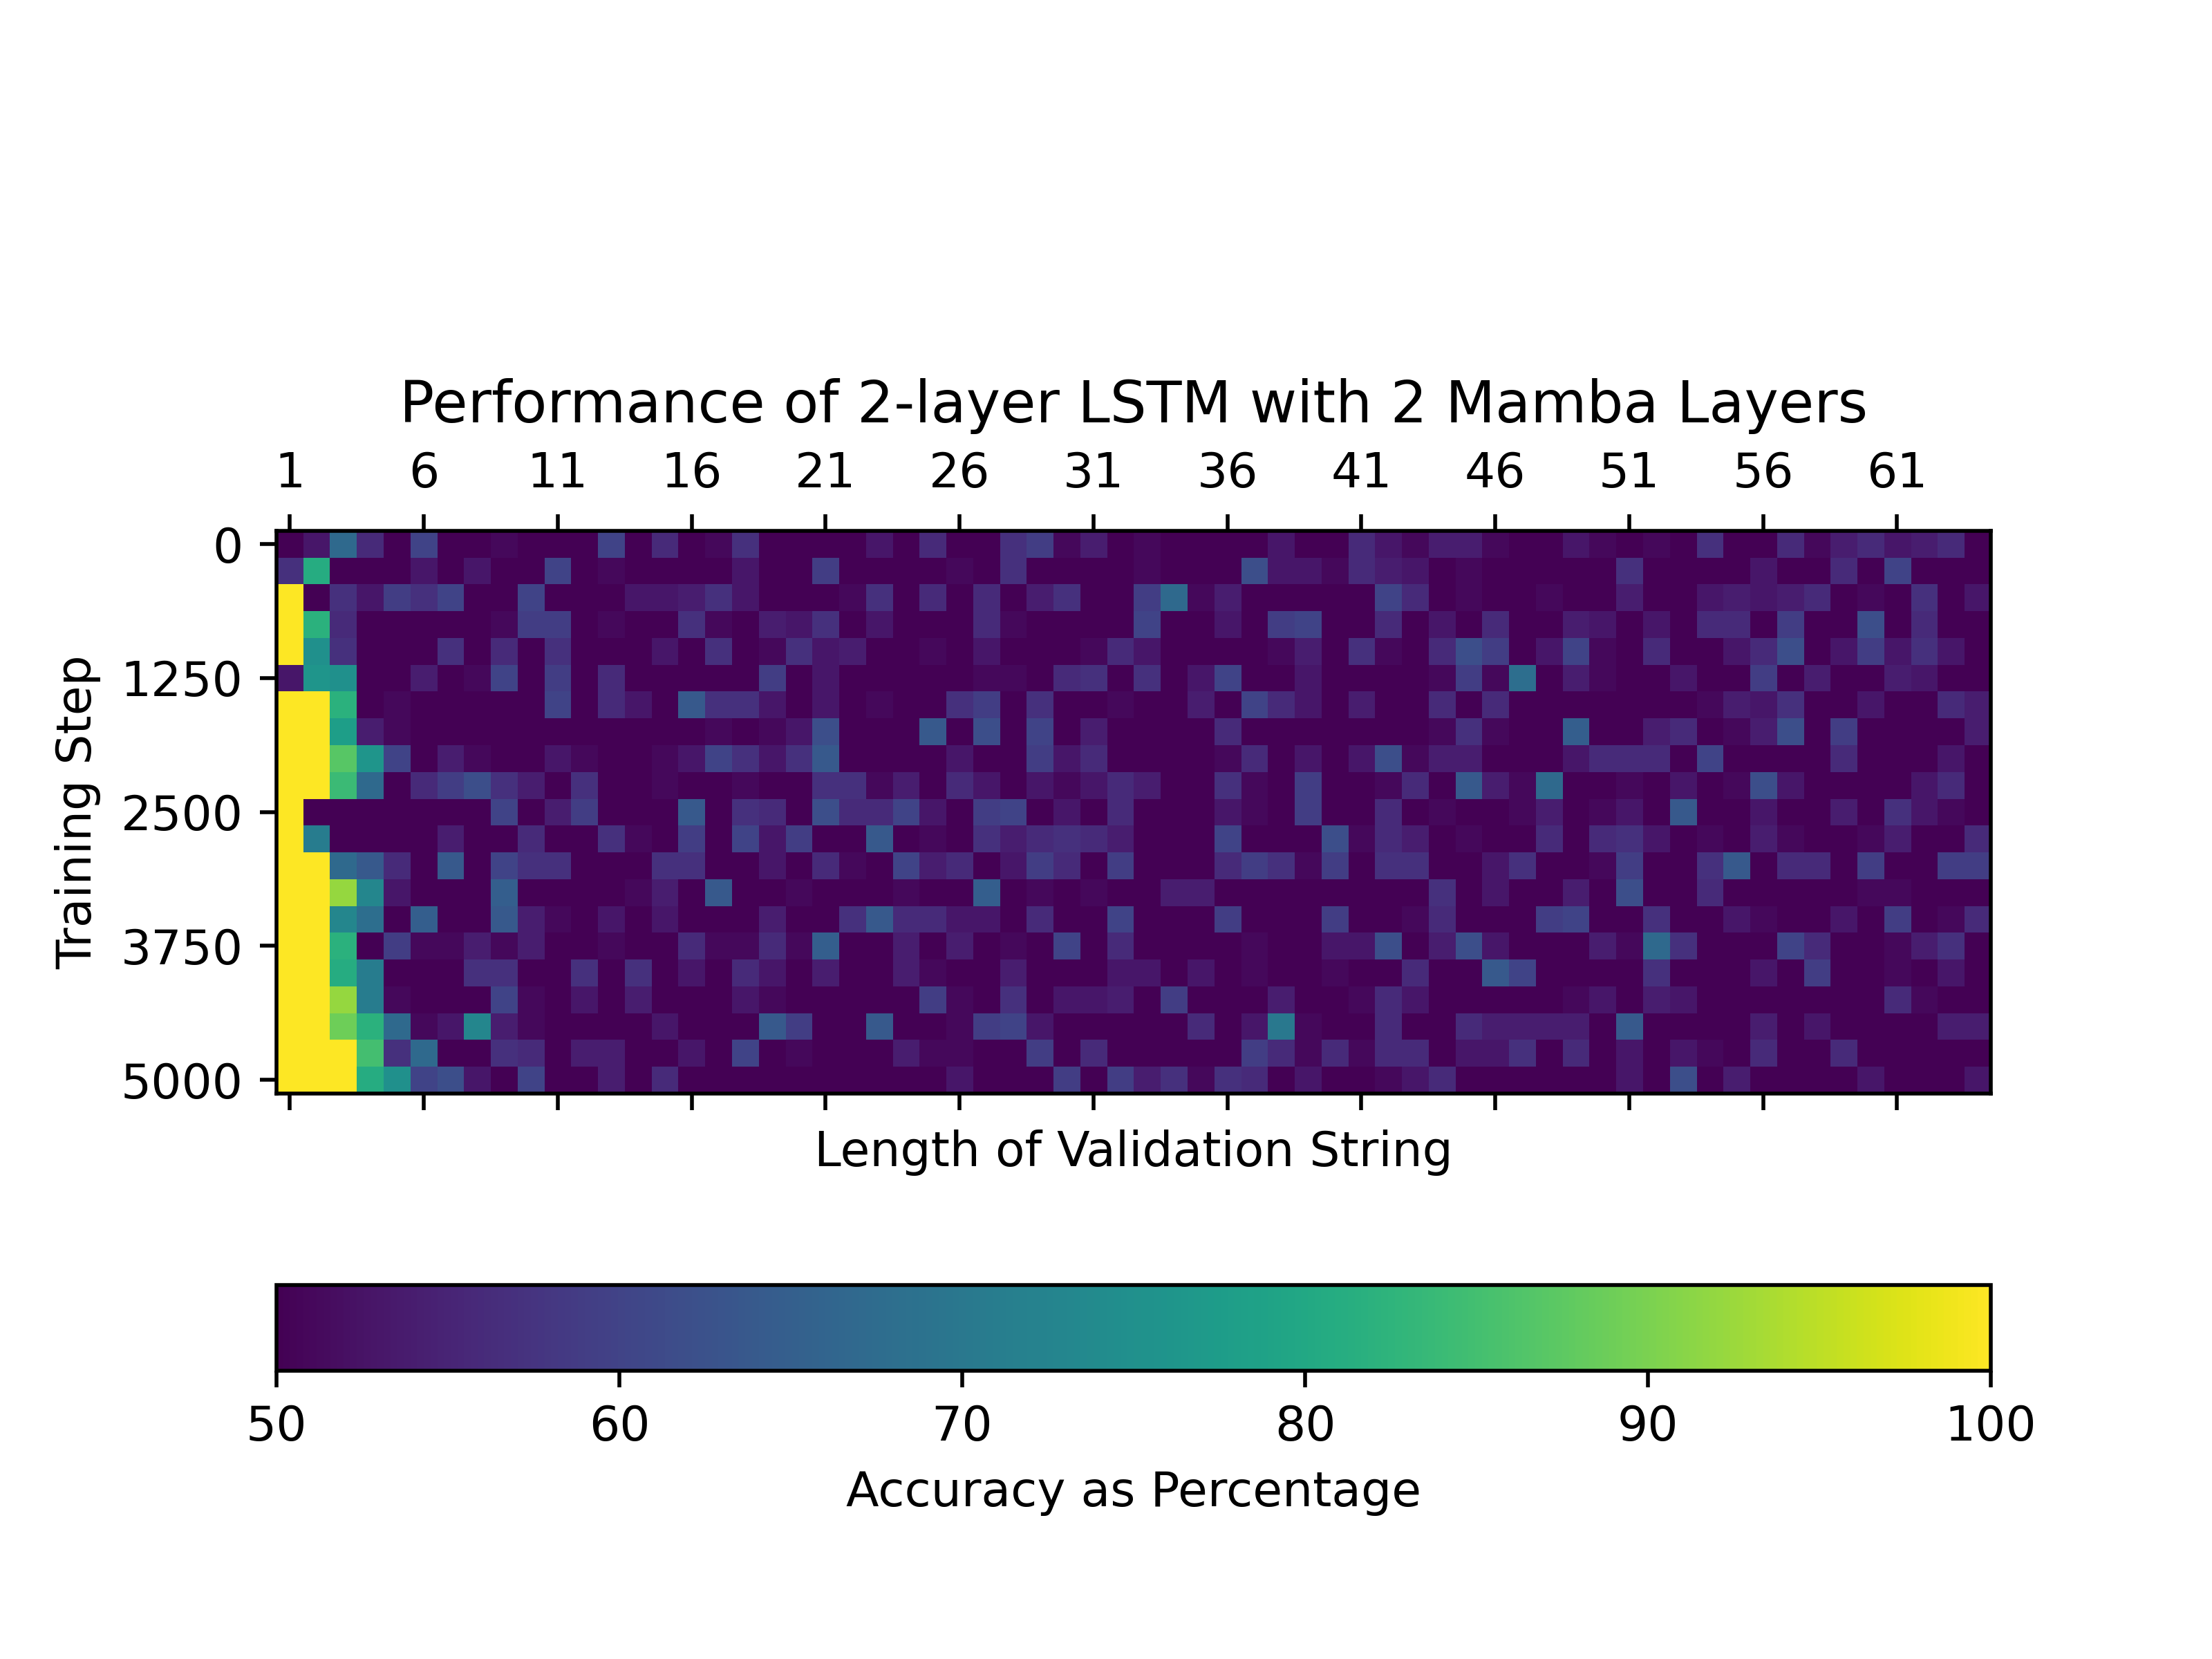
\includegraphics[width=0.8\textwidth]{figures/parity_lstm_False_4_2.png.png}
        \end{center}
    \end{subfigure}\begin{subfigure}{0.5\textwidth}
        \begin{center}
        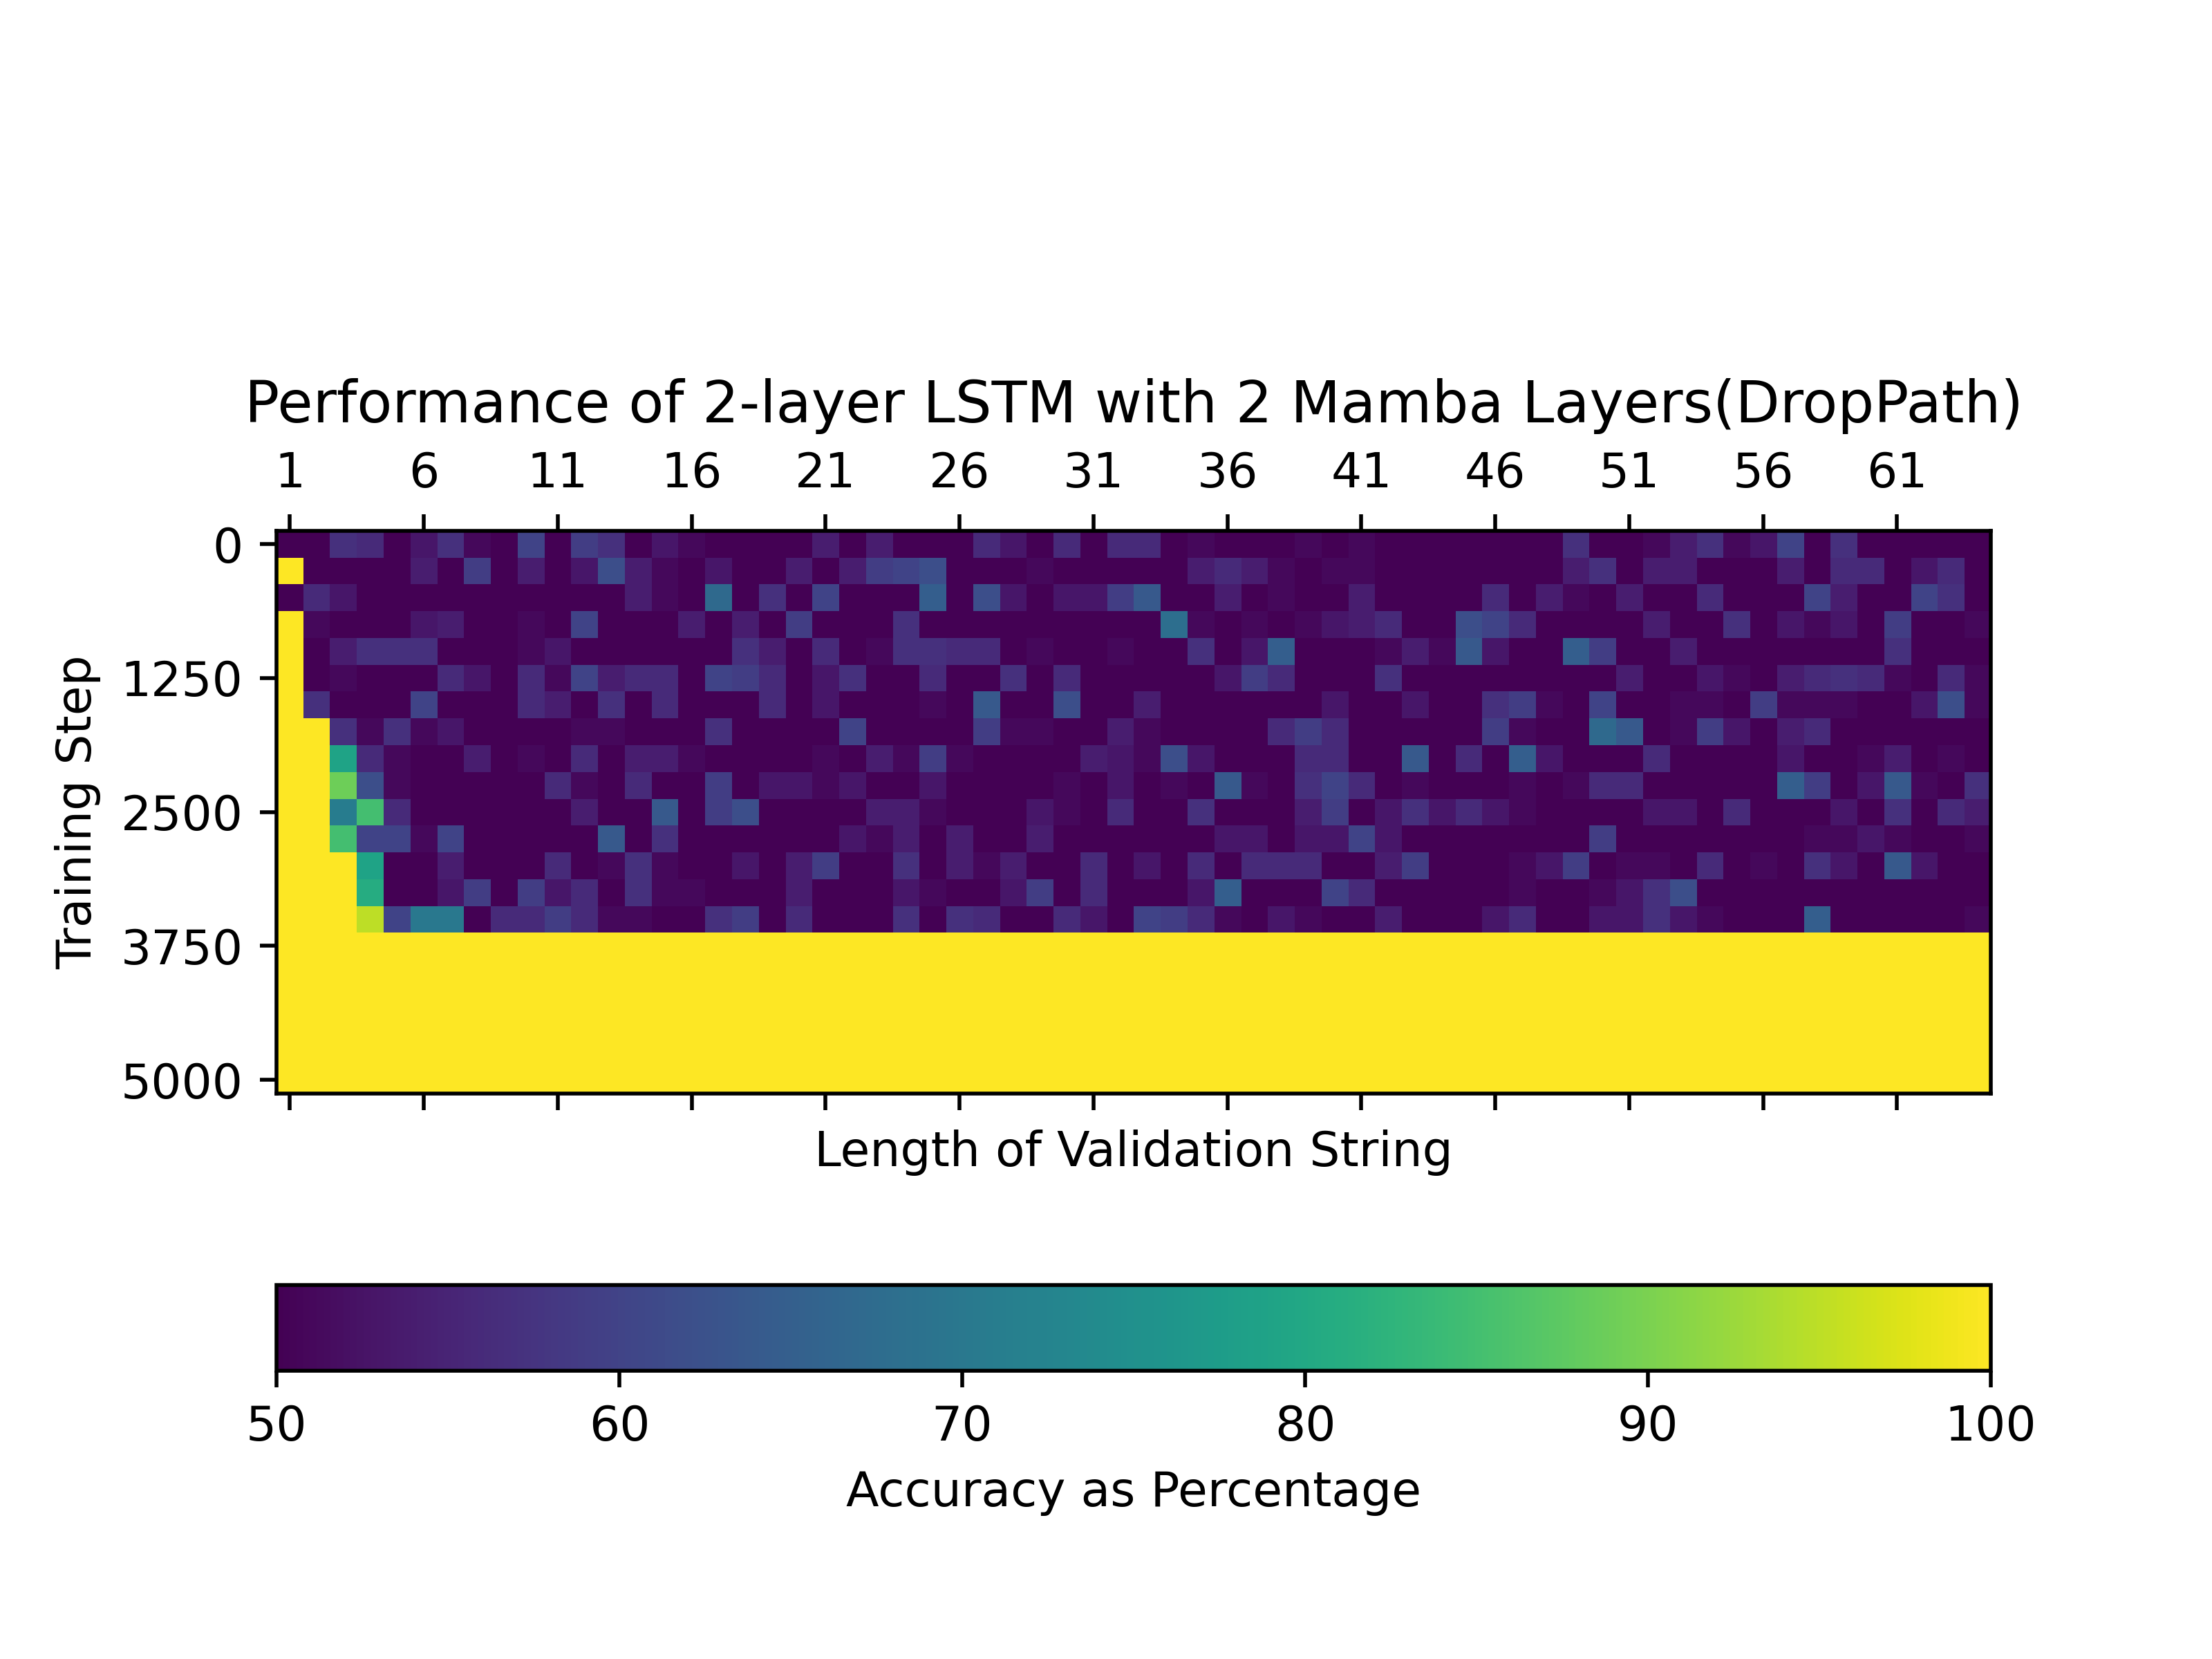
\includegraphics[width=0.8\textwidth]{figures/parity_lstm_True_4_2.png.png}
        \end{center}
    \end{subfigure}
    \begin{subfigure}{0.5\textwidth}
        \begin{center}
        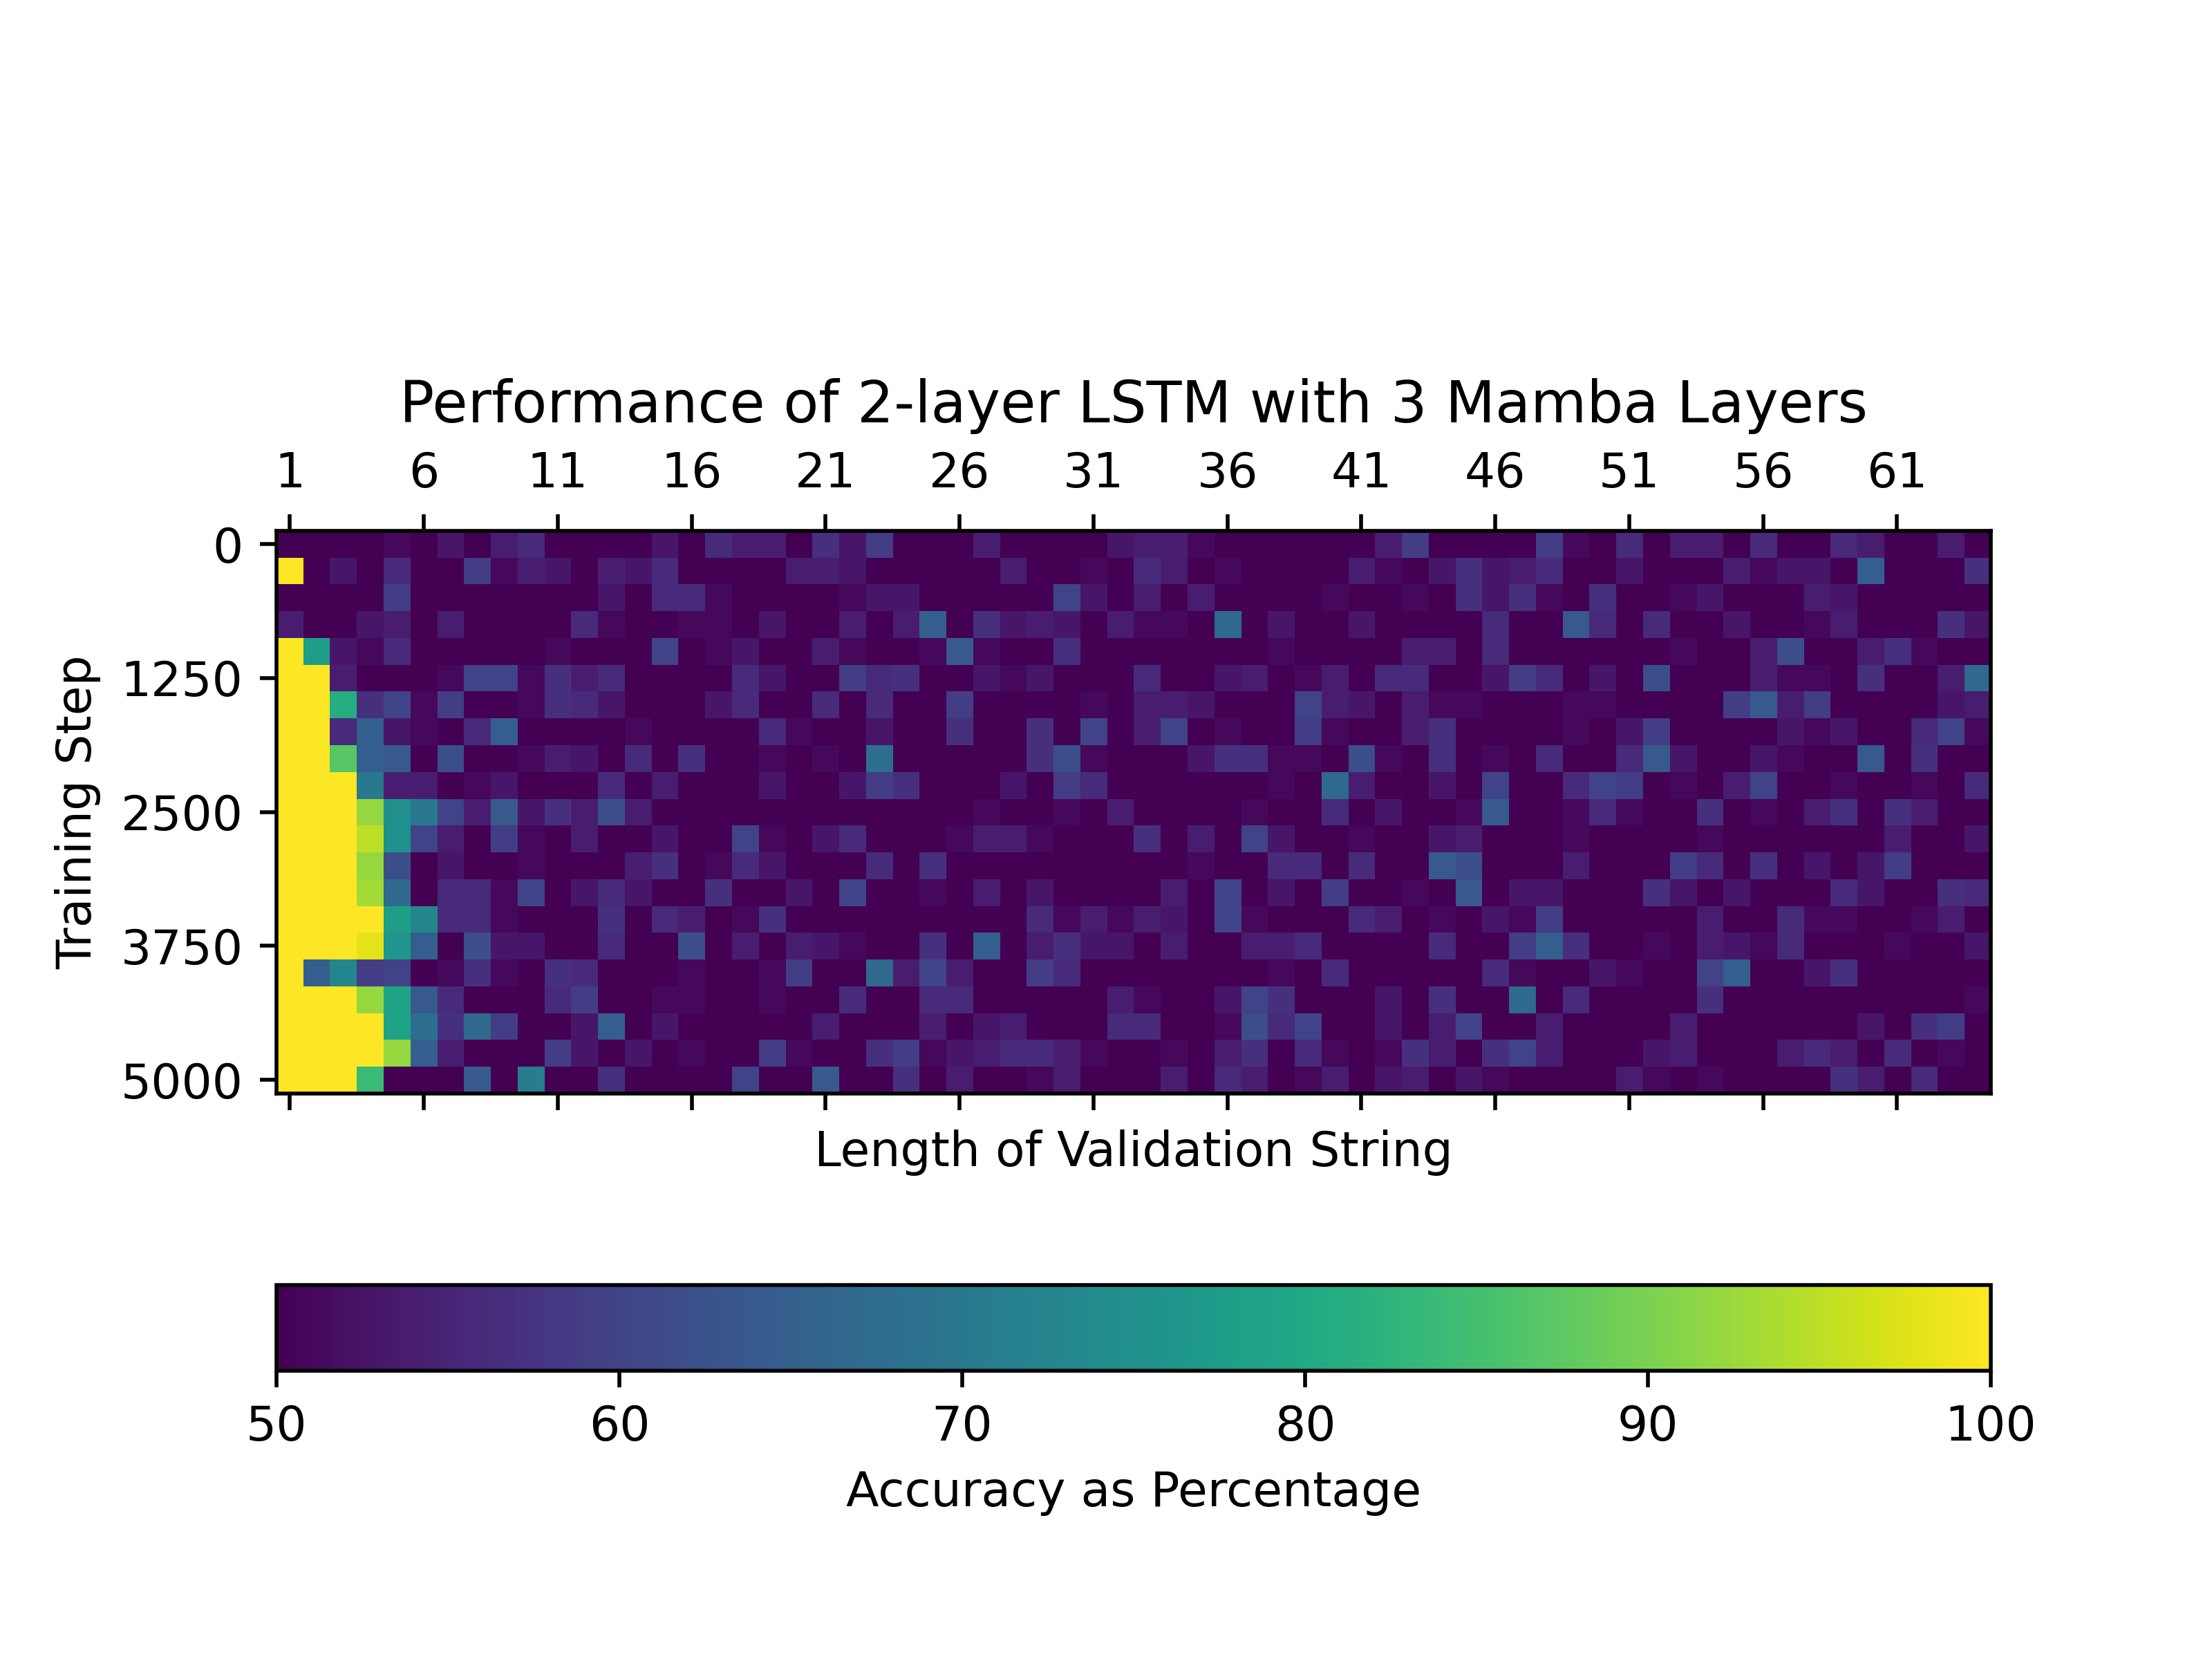
\includegraphics[width=0.8\textwidth]{figures/parity_lstm_False_5_1.png.png}
        \end{center}
    \end{subfigure}\begin{subfigure}{0.5\textwidth}
        \begin{center}
        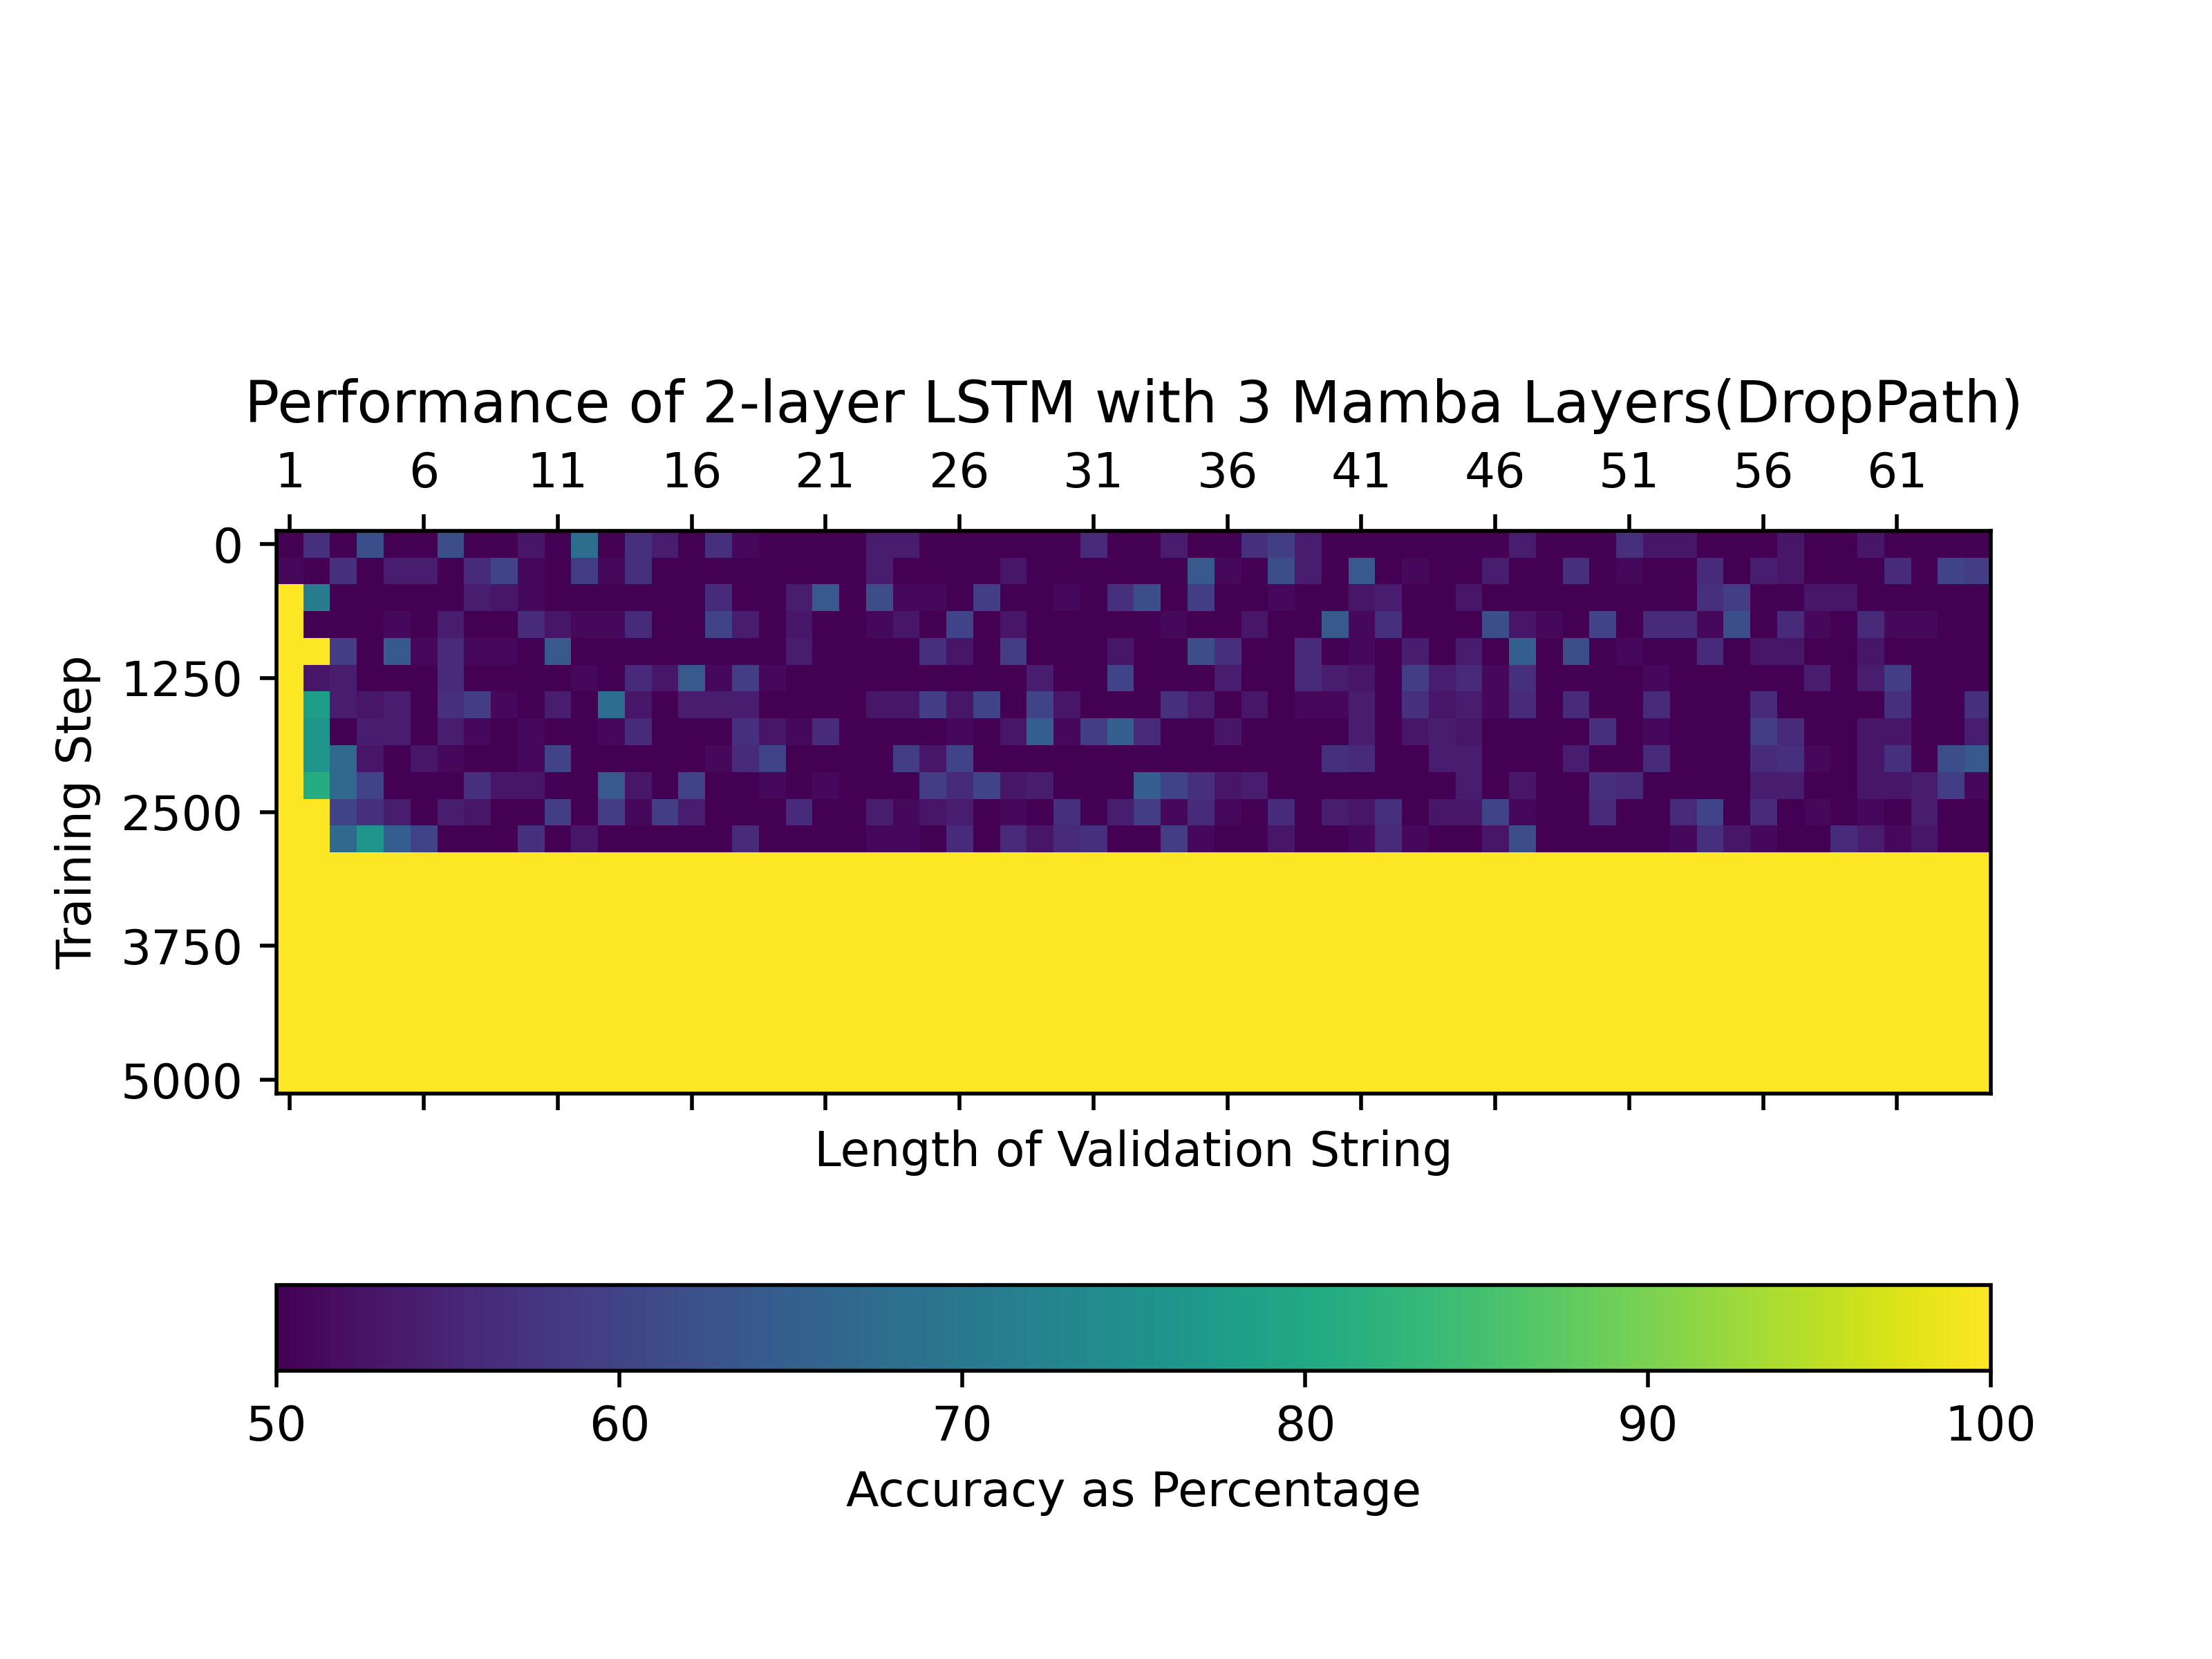
\includegraphics[width=0.8\textwidth]{figures/parity_lstm_True_5_1.png.png}
        \end{center}
    \end{subfigure}
    \begin{subfigure}{0.5\textwidth}
        \begin{center}
        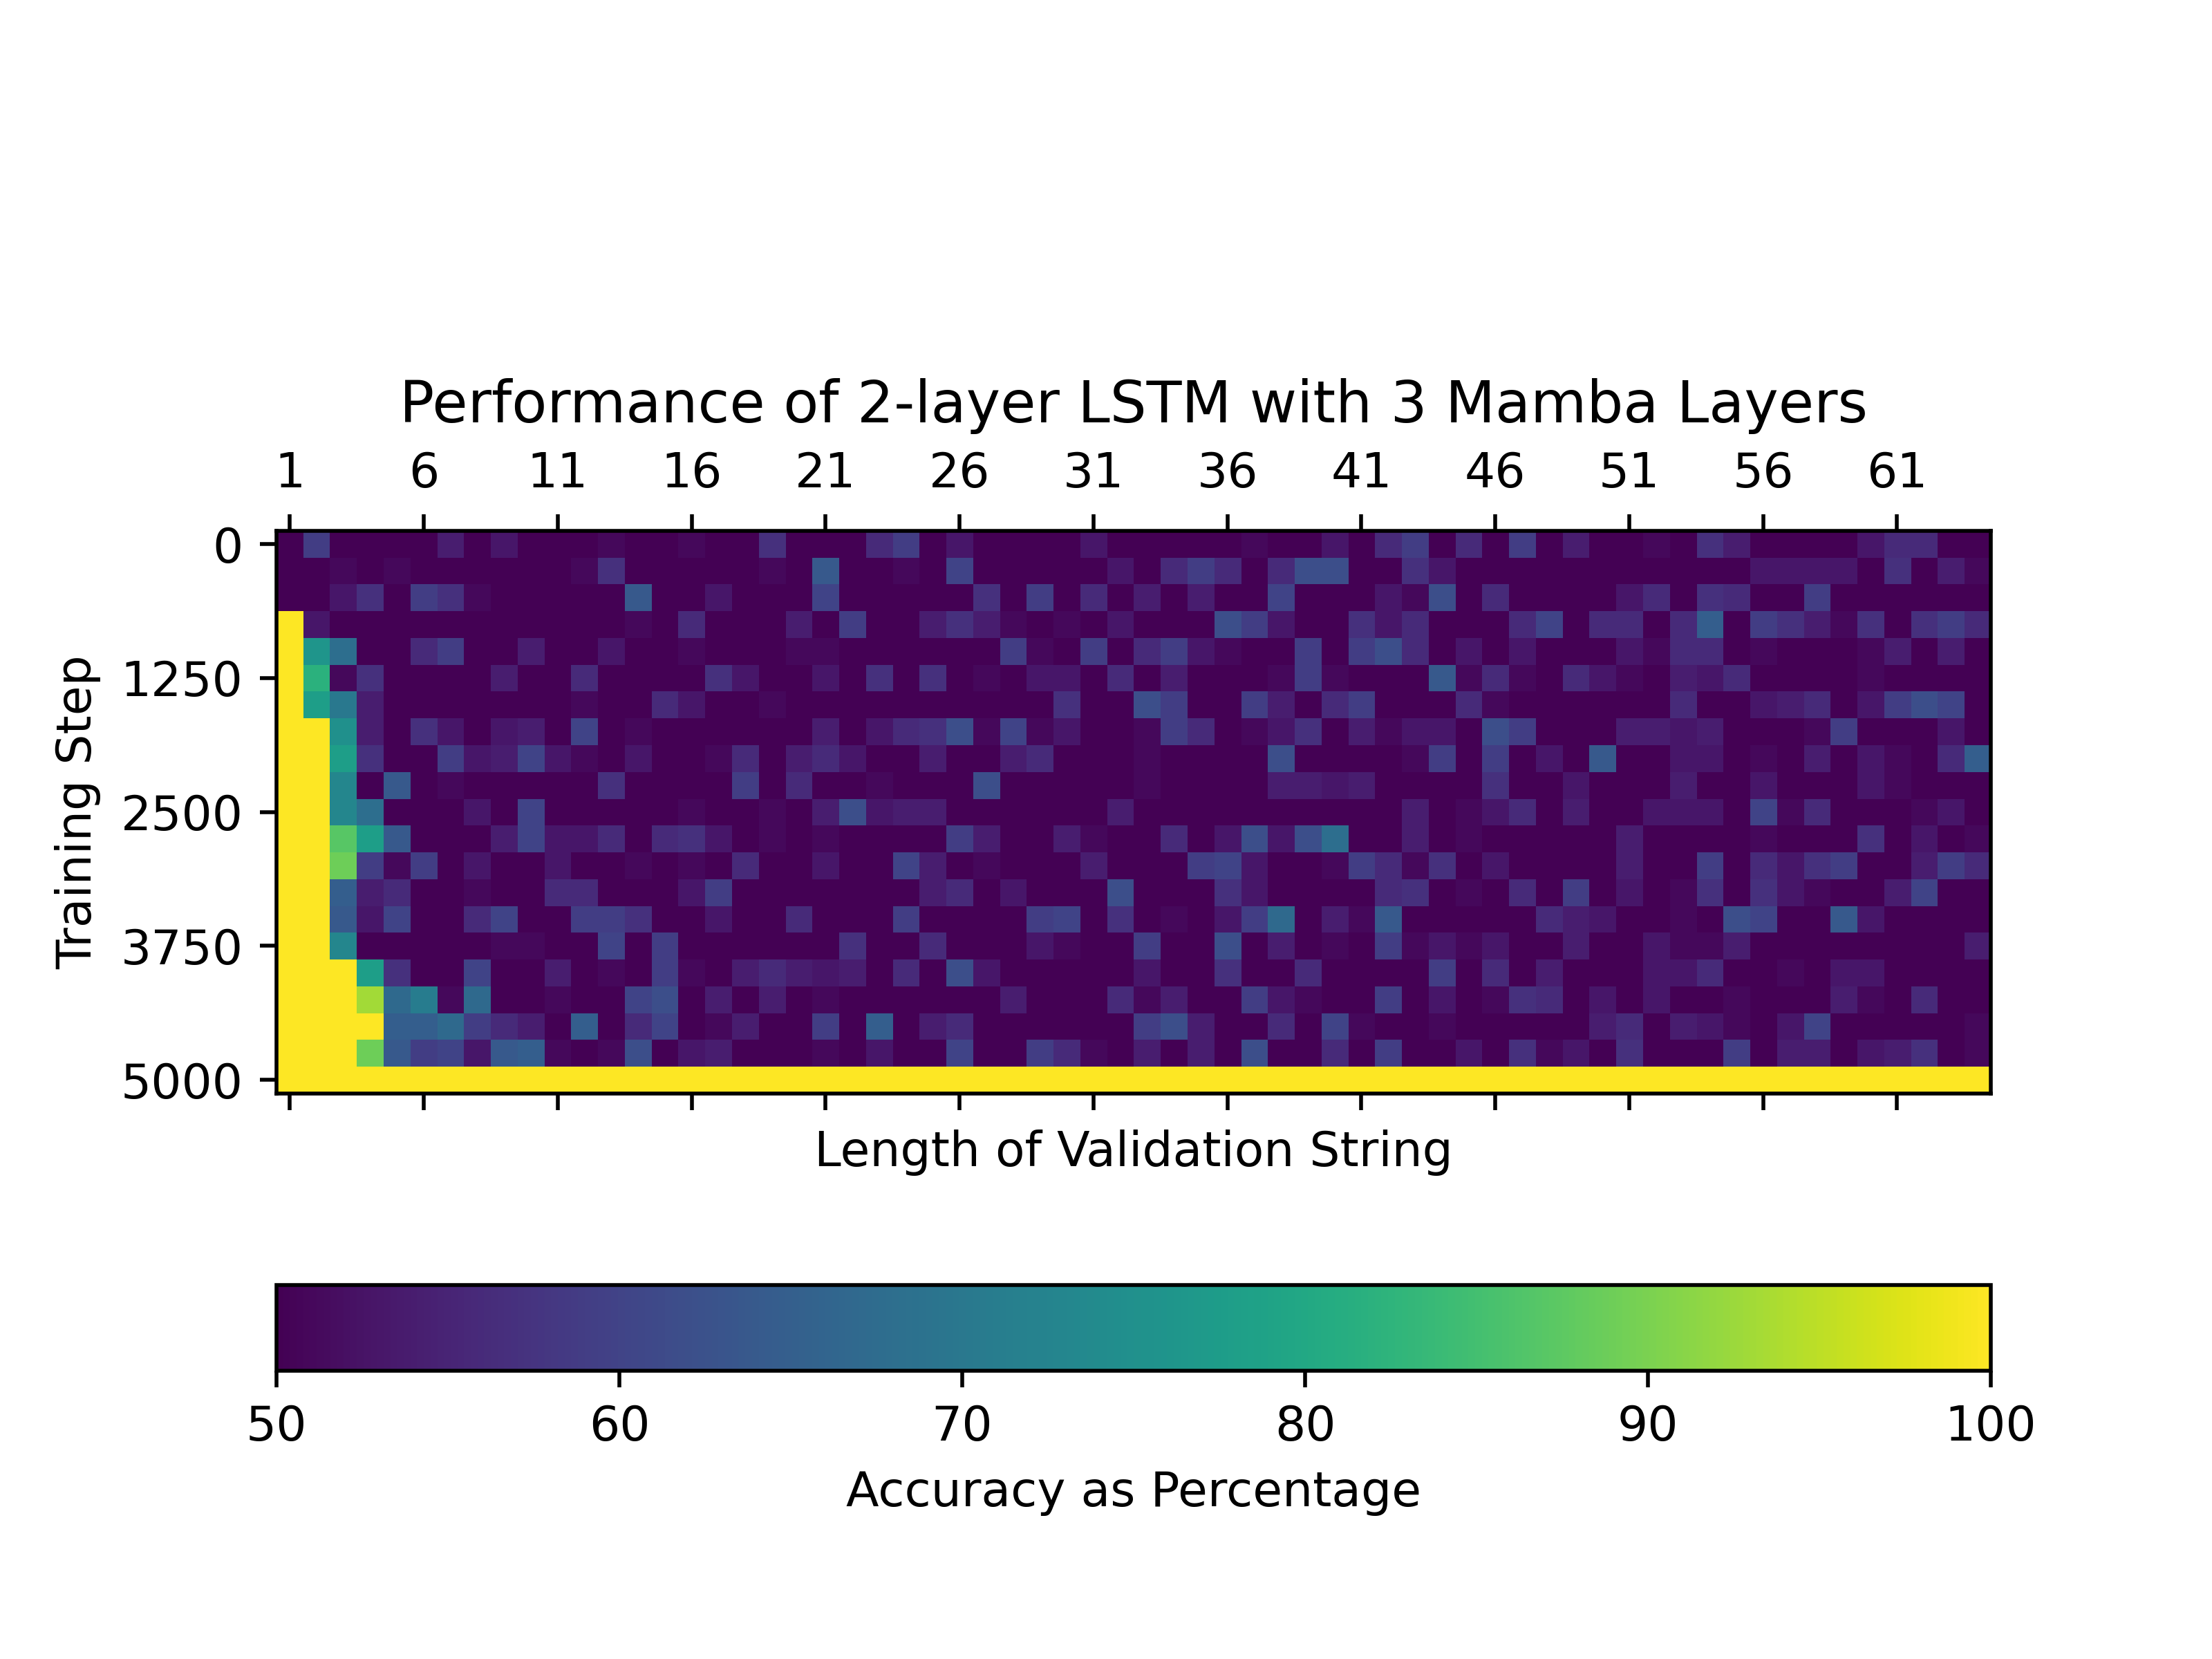
\includegraphics[width=0.8\textwidth]{figures/parity_lstm_False_5_2.png.png}
        \end{center}
    \end{subfigure}\begin{subfigure}{0.5\textwidth}
        \begin{center}
        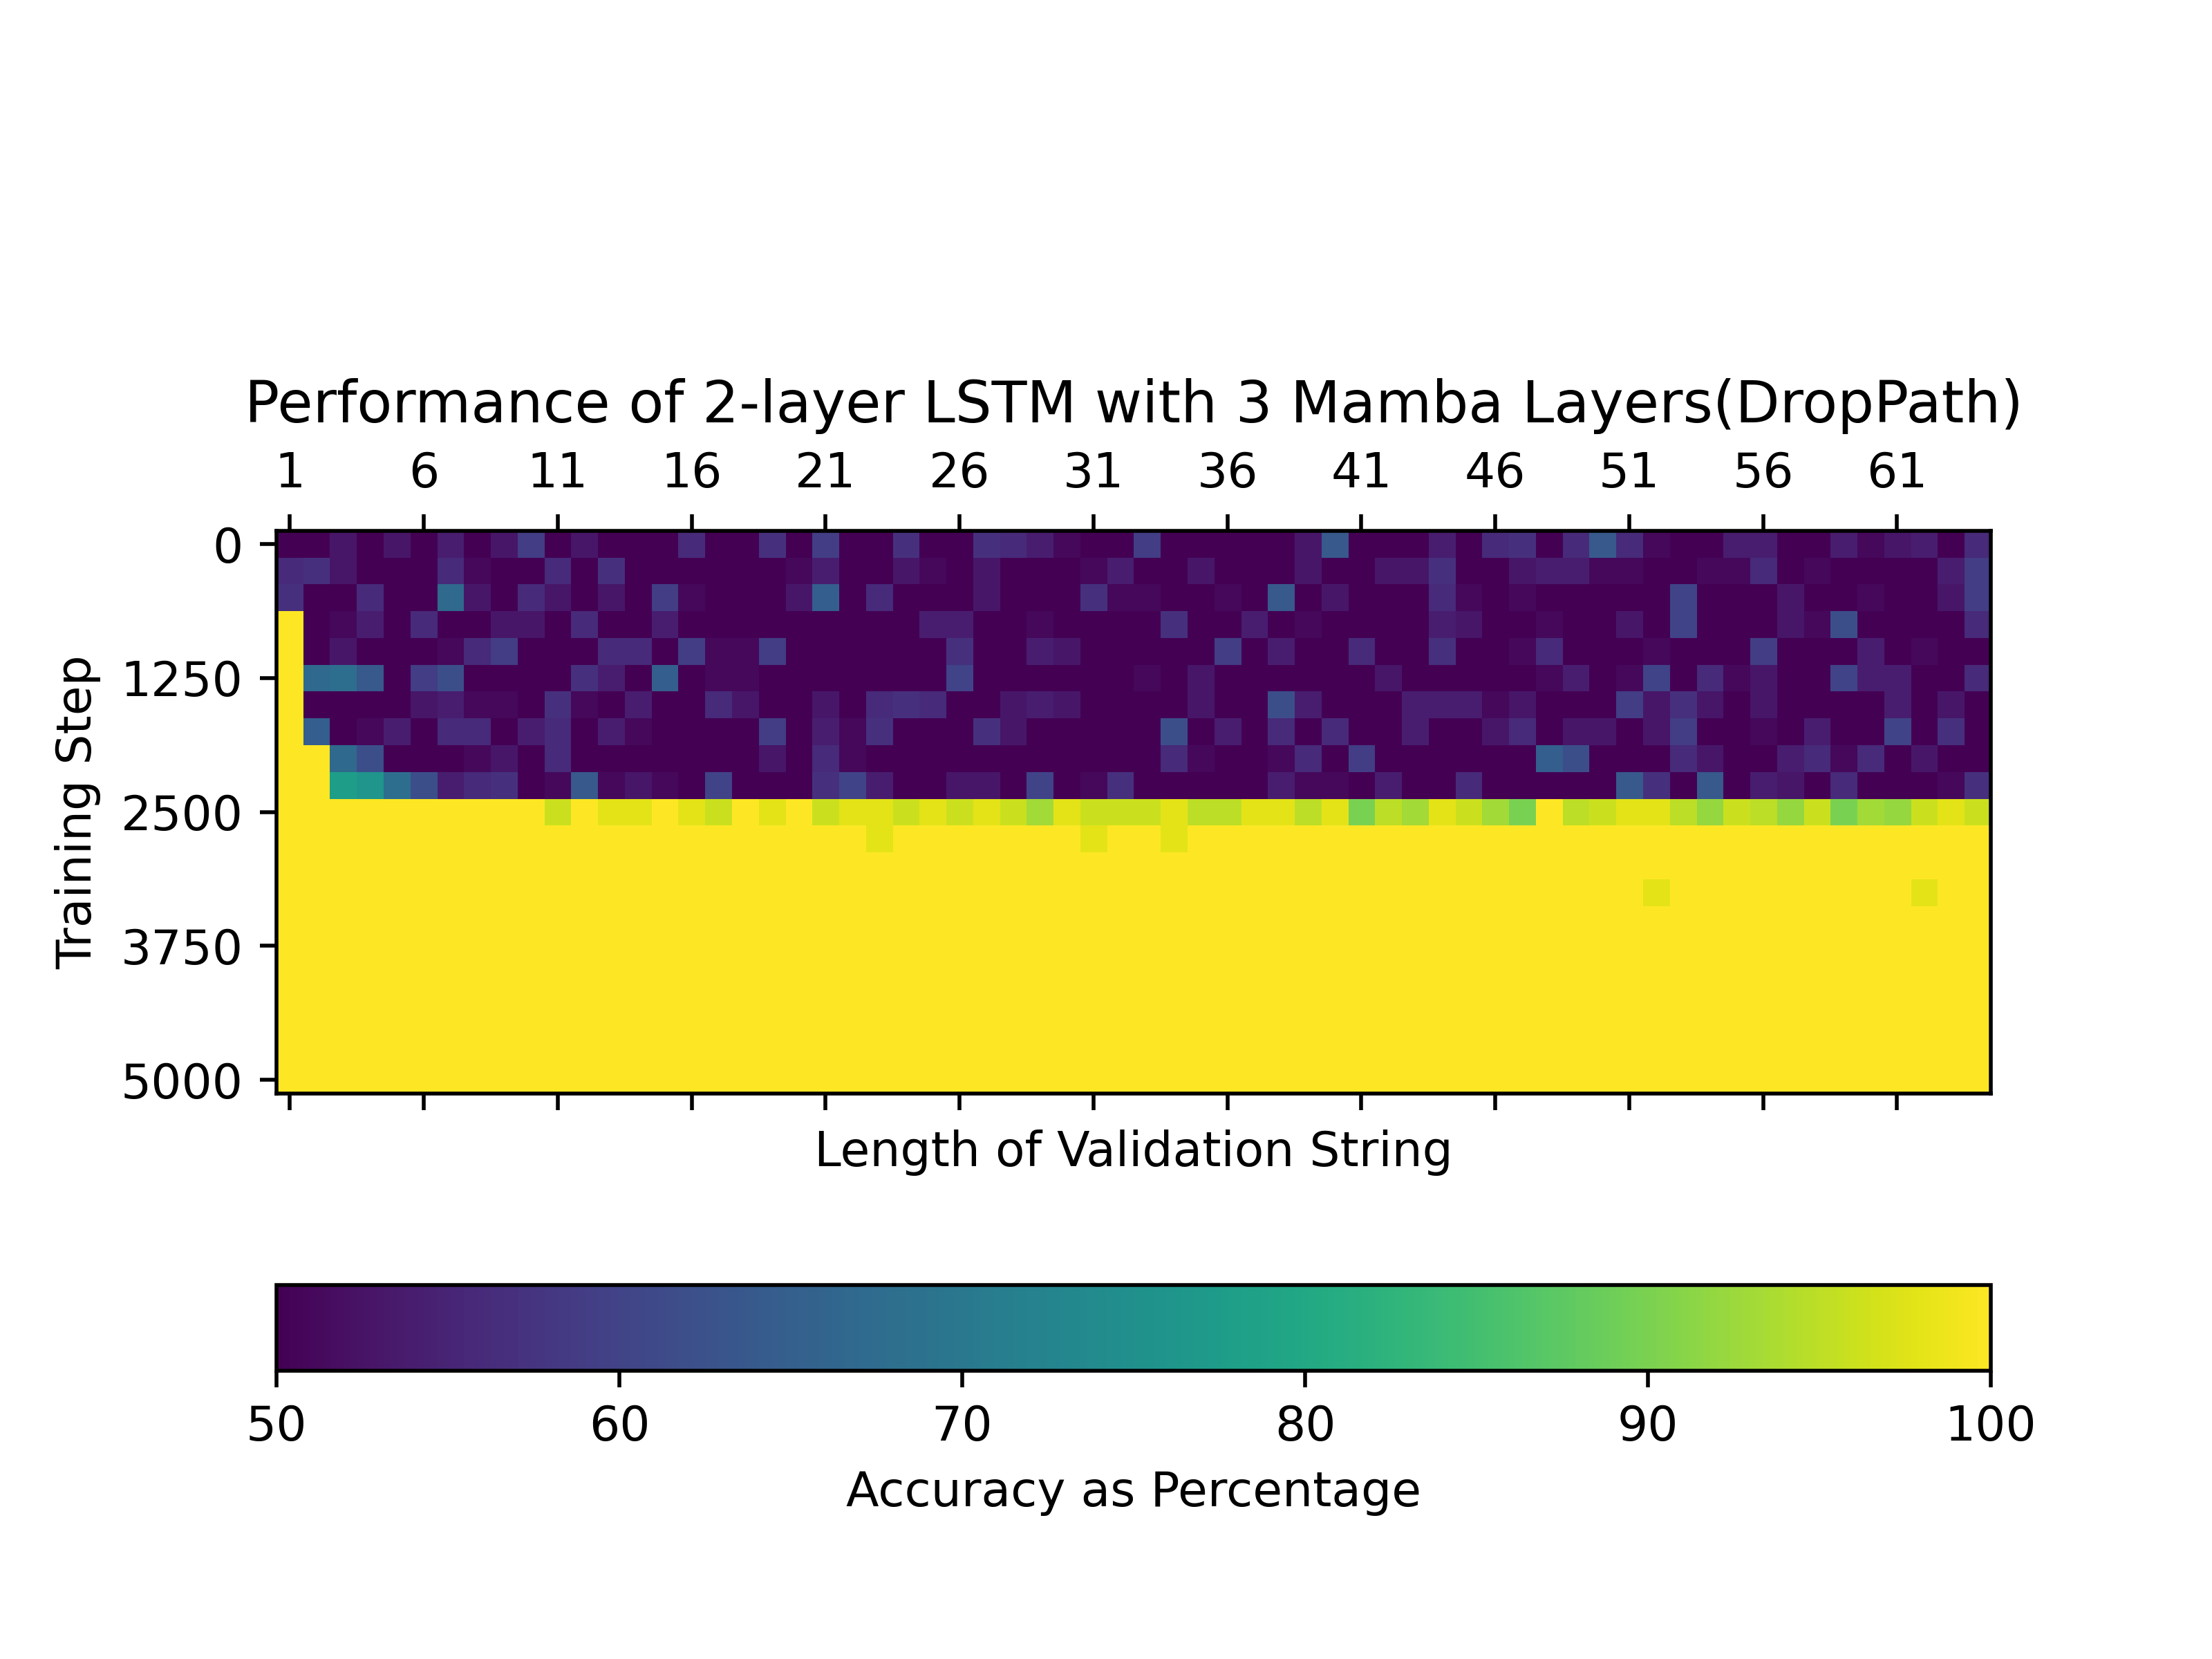
\includegraphics[width=0.8\textwidth]{figures/parity_lstm_True_5_2.png.png}
        \end{center}
    \end{subfigure}
    \caption{Results for parity}
    \label{droppathresults}
\end{figure}
as shown in Figure \ref{droppathresults}, all of the stacks with droppath
generalized within 5000 training steps, while only 3 of the 6 runs generalized
without Drop Path.

\subsection{Ability to recognize CFGs}
An interesting finding from the literature is that despite not being able to
recognize all regular languages, Mamba is theoretically capable of recognizing
some CFGs. For instance, SSMs are theoretically capable of recognizing any Dyck
language by implementing internal counters.

An important component of many CFG-related operations is matching strings to
non-terminal symbols.
As such, we devise a test to determine Mamba's ability 

% ARITHMETIC

\begin{figure}
    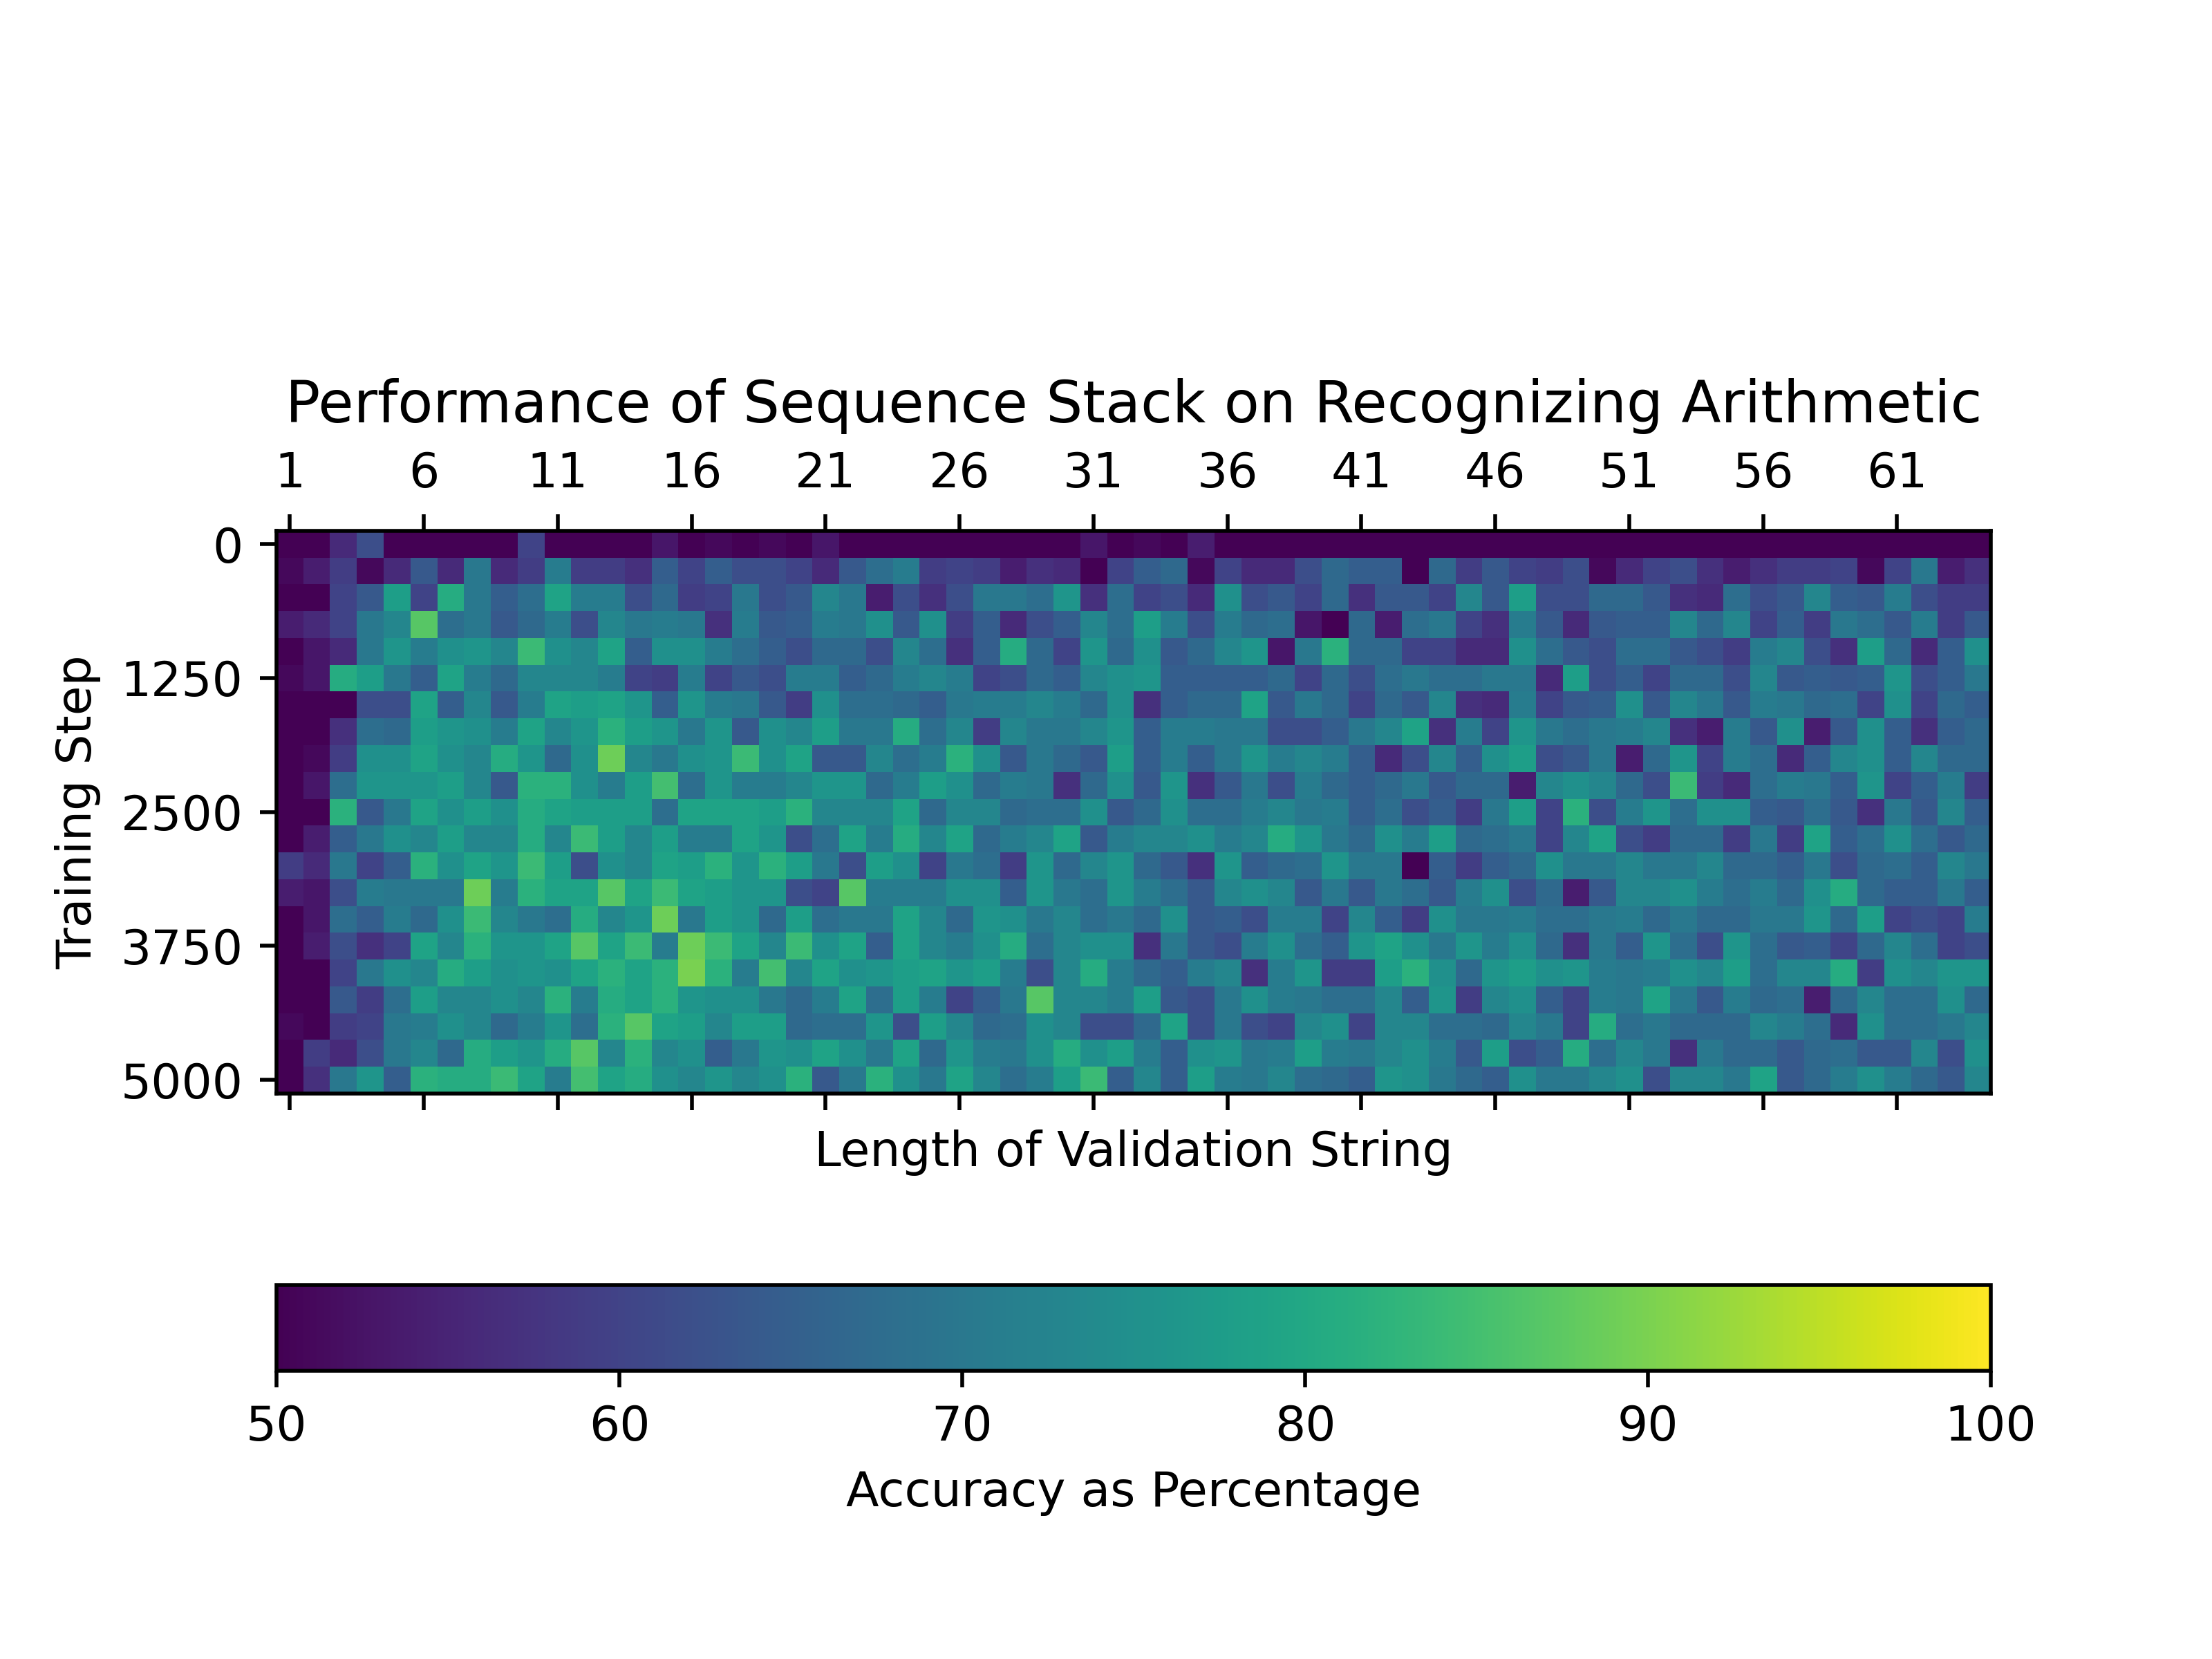
\includegraphics[width=\textwidth]{figures/arithmetic.png}
    \caption{}
    \label{resultsarithmetic}
\end{figure}
In this experiment, we train a multi-layer Mamba model to distinguish 2
non-terminal symbols in the following CFG:
\begin{verbatim}
    G := E
    E := T
    E := E+T
    T := F
    T := T*F
    F := X
    F := (E)
    X := X'
    X := x
\end{verbatim}
This is the CFG for valid arithmetic expressions.
For instance, \verb|(x'+x)*x'| is a valid string in this language while
\verb|x'+x)| is not.

We train a multi-layer model to distinguish the non-terminal symbols E and T.
This requires the model to detect 
Since \verb|T| is a subset of \verb|E|, we don't expect the model to perform
perfectly on this task.

\textbf{Model}
The model we use is the same model as in our \texttt{a|bb+} recognizer. We use
the following hyperparameters:
\begin{verbatim}
  mamba_d_model=16
  d_intermediate=16
  mamba_d_state=256
  mamba_d_conv=4
\end{verbatim}

\textbf{Dataset}
The dataset that we use is a synthetic dataset where each instance is generated
as follows:
\begin{itemize}
    \item Choose a random length in the range 1 to 64 inclusive
    \item Choose a random non-terminal: 50\% G, 50\% T
    \item Derive a random string with the given length
\end{itemize}
We generate 5000 batches, with 64 instances per batch.
The derivation step is done efficiently using a dynamic programming algorithm.

\textbf{Training}
We train the model for 1 epoch using Adam.
Our learning rate is $10^{-3}$.

\textbf{Results}
As shown in Figure \ref{resultsarithmetic}, the model learns to distinguish the
2 languages with around 70\% accuracy across all string lengths.

\begin{figure}
    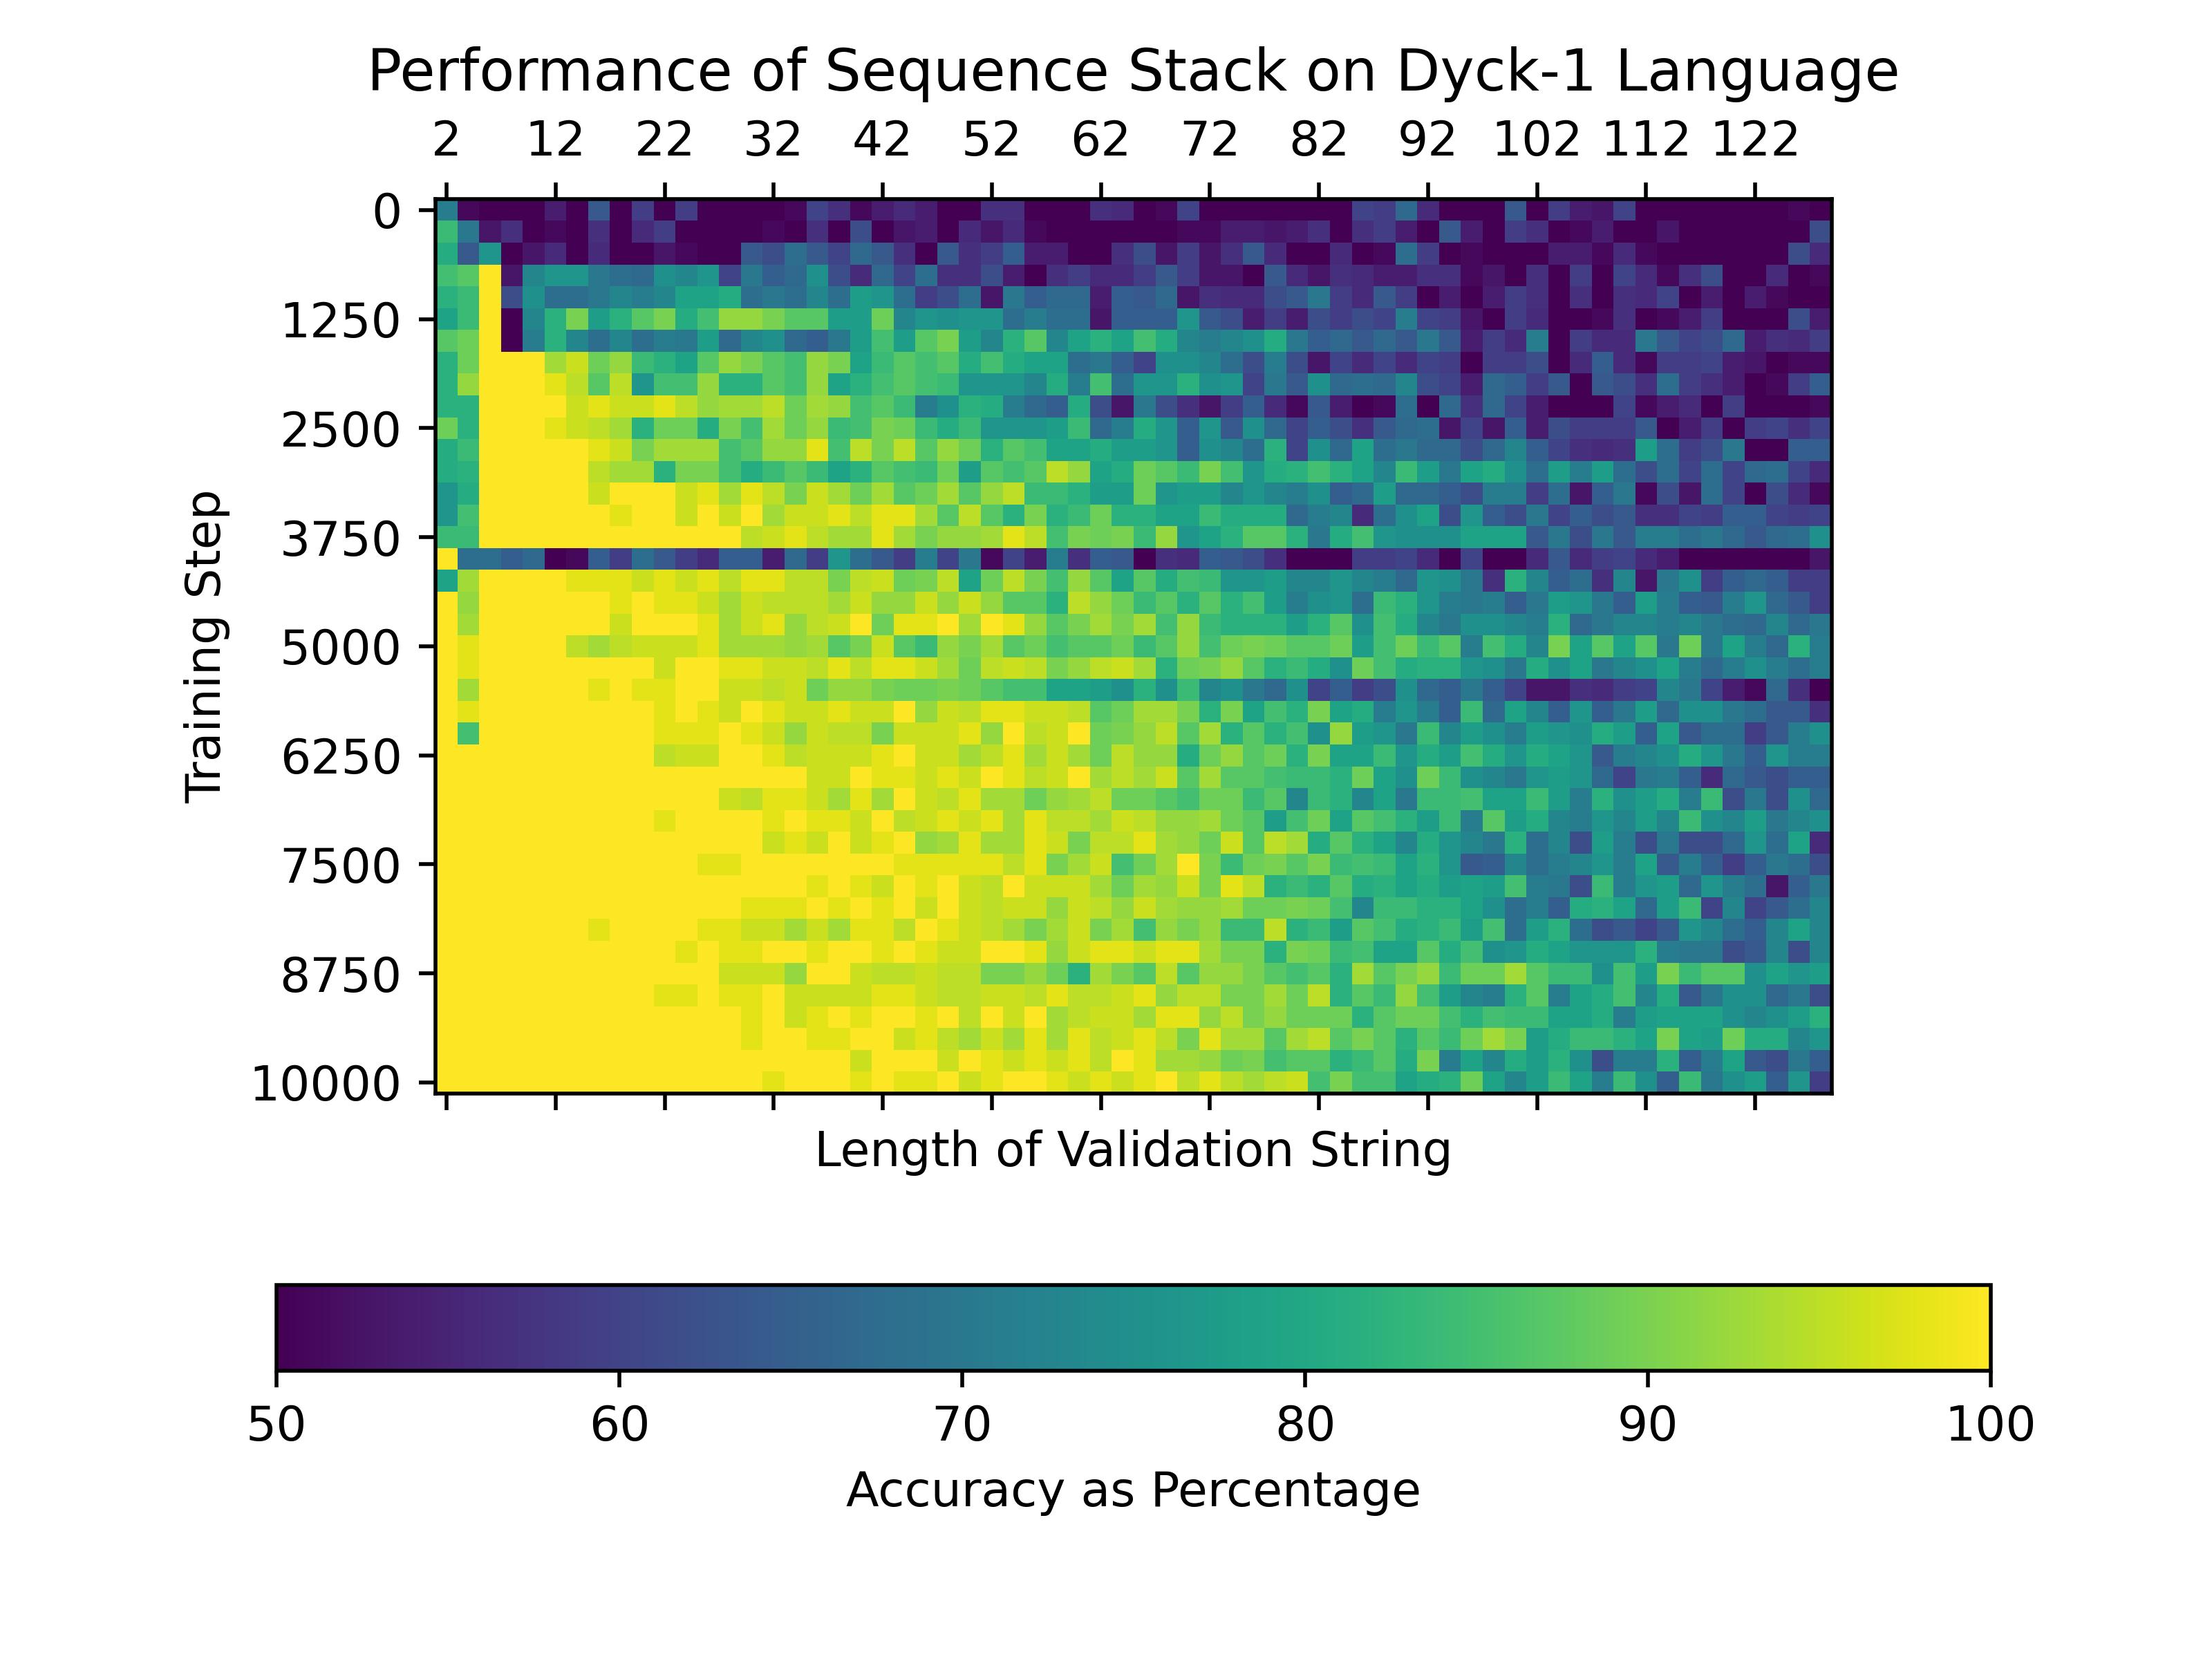
\includegraphics[width=\textwidth]{figures/dyck.png}
    \caption{}
    \label{resultsdyck}
\end{figure}
\begin{figure}
    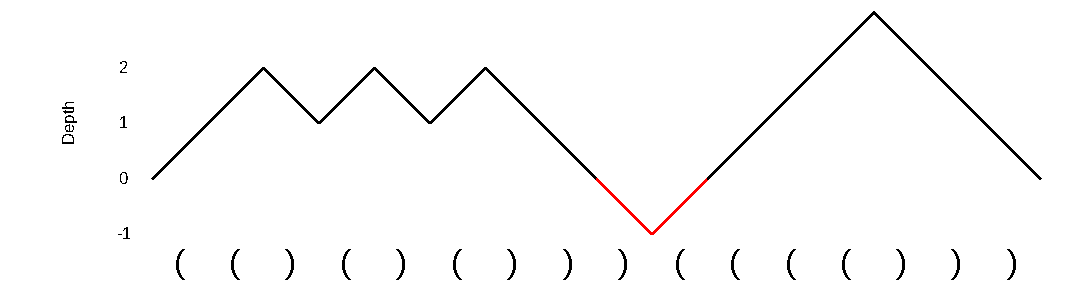
\includegraphics[width=\textwidth]{figures/dyck_challenge.pdf}
    \caption{}
    \label{dyckchallenge}
\end{figure}

\subsection{Dyck-1}
One specific CFG that is well studied is the Dyck family of languages.
A previous paper\cite{ssmformal} has found that multi-layer Mamba architectures
claims to experimentally confirm that multi-layer Mamba is capable of
recognizing Dyck-1 strings. However, they sweep through a set of hyperparameters
such that the largest total state size is many times the length of their
validation samples: in their tests on Dyck-1, their maximum state size is 256
dimensions while their longest validation string is 100 characters long.
In addition, they don't reveal the hyperparameters used to get achieve the
results that they got.
In this section, I reproduce their finding using a much smaller model.

\textbf{Model}
The model that we use is identical to the multilayer Mamba model described in
the first experiment.
The hyperparameters that we use are:
\begin{verbatim}
  n_layer=2
  d_intermediate=64
  mamba_d_model=4
  mamba_d_state=2
  mamba_d_conv=2
\end{verbatim}
The total state dimension is given by
$$
n_layer * d_model * (d_state + d_conv - 1) = 24
$$

\textbf{Dataset}
The dataset that we use is an even split between Dyck-1 instances and
"difficult" non-instances(explained in the next paragraph).
The string lengths are evenly distributed among the even numbers from 2-64
inclusive and the two classes are evenly split as with the previous instances.
We generate 10000 batches with 64 instances per batch.
The validation set is 2-128 instead of 2-64 to test generalization.

To explain what "difficult" non-instances are, it's first important to
understand the rules for valid Dyck-1 strings.
Dyck-1 strings are equivalent to matched strings of parentheses.
The validity of a string can be calculated by scanning along the string and
tracking the "depth" at each character. The character \verb|(| increases the
depth, since it enters a pair. The character \verb|)| decreases the depth, since
it exits a pair.
If the depth is never negative, and the final depth is 0, then the string is
valid.
A difficult string ends at a depth of 0, and only has a negative depth of -1 at
one point near the middle.
This ensures that any counter-based recognizer needs to be numerically precise,
since a small error can prevent the model from recognizing the small negative
region.
An example of such a string is shown in Figure \ref{dyckchallenge}

\textbf{Results}
As shown in Figure \ref{resultsdyck}, the smaller model is able to achieve
better-than-chance results on strings twice the length of its training data.
This is shows that multi-layer Mamba is able to track depths significantly
larger than its state size, which provides a strong piece of evidence that
the model is using a literal depth counter in to evaluate strings.

\subsection{Conclusion of Exploratory Section}
Overall, we've learned some features of Mamba that will be pretty useful for
model design.
We've learned that the Mamba architecture has a strong inductive bias for
fixed pattern-matching.
We also learned that the Mamba architecture tends to perform better with gating
and other mechanisms to isolate it from the rest of the model.
Although not useful to our own endeavors, we've confirmed an interesting
theoretical result about Mamba's expressive capacity.
